\documentclass[12pt,a4paper]{scrartcl}
\usepackage[utf8]{inputenc}
\usepackage{amsmath}
\usepackage{amssymb}
\usepackage{braket}
\usepackage{amssymb}
\usepackage{graphicx}
\usepackage{float}
\usepackage{wrapfig}
\usepackage{dsfont}
\usepackage{enumitem}
\usepackage{subfig}
\usepackage[top=3cm, left=3cm, right=3cm, bottom=3cm]{geometry}
\usepackage{fancyhdr}
\usepackage{sidecap}
\usepackage{pstricks}
\usepackage{mathrsfs}
\usepackage{listings}
\usepackage[absolute]{textpos}
\numberwithin{equation}{section}
%\numberwithin{figure}{section}
%\usepackage[pdfborder=0 0 0]{hyperref}
\usepackage[colorlinks=True, urlcolor=blue]{hyperref}
\pagestyle{fancy}
\fancyhead[C]{}
\fancyhead[L]{}
\fancyfoot[C]{\thepage}
\fancyhead[R]{}

\newcommand{\cng}[1]{{\color{red}#1}}
\newcommand{\sgn}{{\mathrm{sgn}}}
\newcommand{\GF}{Green's function}
\newcommand{\unity}{\mathds{1}}
\renewcommand{\vec}{\mathbf}

\title{GW (oneshot) + DMFT documentation}

\begin{document}
\maketitle
\tableofcontents


\section{Introduction}

This document  provides the prescription of the combination of a GW calculation
for correlated materials with DMFT applied only to a subset of correlated orbitals.
At this level, the GW calculation will be performed only once at the beginning (one-shot)
based on a DFT Hamiltonian $H^{DFT}$,
to obtain a nonlocal Selfenergy $\Sigma^{GW}$ for all states. 
In addition, the local part of $\Sigma^{GW}$ of a subset of strongly correlated orbitals will be replaced by a Selfenergy $\Sigma^{DMFT}$
obtained within a selfconsistent DMFT scheme, 
where the selfconsistency is done including the full nonlocal
effects of the combined Selfenergy.

No further selfconsistency apart from the DMFT cycle will be performed, {\it i.e.} no update of $\Sigma^{GW}$ will be done. By this, the final interacting system will be
described by a {\GF} with the non-interacting DFT dispersion, corrected by a non-local Selfenergy where the non-local components
correspond to $\Sigma^{GW}=G_0W_0$, while the local components
of the correlated orbitals correspond to $\Sigma^{DMFT}$.
This $\Sigma^{DMFT}$ is usually different to the one obtained by
a standard DMFT calculation since the selfconsistency is
done with the inclusion of the nonlocal parts of the 
Selfenergy.

Extensions to a full GW+DMFT selfconsistency will be discussed elsewhere.

\section{Approximation to the free energy functional $\Gamma[G,W]$: Combination of GW and DMFT}
As stated by Almbladh[ref], the free energy of a solid can be written in terms of
a functional $\Gamma[G,W]$ of the fully dressed Green's function $G$
and the screened Coulomb interaction $W$. While an analytic expression for 
$\Gamma$ is not known, it can be shown that it can be separated into 
a Hartree part $\Gamma^H$ and a correction arising from all other many-body effects
$\Psi$
\begin{align}
\Gamma[G,W] &= \Gamma^H[G,W] + \Psi[G,W].
\end{align}
The many-body correction $\Psi[G,W]$ is the sum of all skeleton diagrams that are
irreducible with respect to both one-electron propagator and
interaction lines. It has the properties
\begin{align}
\frac{\delta \Psi}{\delta G} &= \Sigma^{XC}  \label{eq:sigma_from_psi} \\
\frac{\delta \Psi}{\delta W} &= -\frac{1}{2}P \label{eq:p_from_psi},
\end{align}
where $\Sigma^{XC}$ is the exchange-correlation Selfenergy corresponding to the
fully dressed Green's function $G$, thus excluding the Hartree part $\Sigma^H$.
$P$ is the full polarization of the system that screens the bare Coulomb
interaction $V$ down to the screened interaction $W$.

Since methods like Density Functional Theory already treat the Hartree contribution
from the Coulomb interaction, we are interested in obtaining
an (approximative) expression for the many-body correction $\Psi[G,W]$.

One possibility is the GW approximation, which expands $\Psi[G,W]$ in powers of the
screened interaction $W$ and truncates the series at first order. The resulting expression
is thus
\begin{align}
\Psi[G,W] \approx -\frac{1}{2} \mathrm{Tr}(GWG).
\end{align}
Using equations \eqref{eq:sigma_from_psi} and \eqref{eq:p_from_psi},
we immediately obtain the $GW$ Selfenergy and polarization as
\begin{align}
\Sigma^{GW} &= -GW \\
P^{GW} &= GG.
\end{align}
While this approximation goes well beyond the level of a simple Hartree approximation
and usually treats all states without any separation of spaces,
it is only an expansion up to first order in $W$ and thus justified only when $W$ is
small, i.e. in case of weakly correlated systems. Thus, it is tempting to combine
$GW$ with other methods like DMFT for an improved treatment of correlated systems.

\bigskip

In the GW+DMFT scheme, we first separate the $\Psi$ functional into
its local and nonlocal parts
\begin{align}
\Psi[G,W] &= \Psi_{\mathrm{nonloc}}[G,W] + \Psi_{\mathrm{loc}}[G,W],
\end{align}
\cng{Is this exact?}
where usually the nonlocal part is approximated by $GW$, while the local part is usually approximated by DMFT,
but right now we do not want to decide on a specific method and only focus
on how to separate the local and nonlocal contributions.

We only want to impose one specific condition: First, we work in an orbital separated scheme,
where we separate the full Hilbert space $L+H$ into a correlated subspace $L$ and the remaining subspace $H$.
Then, our defintion of $\Psi_{\mathrm{loc}}$ is the following: $\Psi_{\mathrm{loc}}$ is generated only from the \underline{local}
components of $G$ and $W$ in the \underline{correlated subspace}, i.e.
\begin{align}
\Psi[G,W] &= \Psi_{\mathrm{nonloc}}[G,W] + \underbrace{\Psi_{}[G^{\mathrm{loc},L},W^{\mathrm{loc},L}]}_{\Psi_{\mathrm{loc}}}.
\label{eq:psi_separation_nonloc_loc}
\end{align}
By this, all internal processes contributing to $\Psi_{\mathrm{loc}}$ 
are restricted to the smaller correlated subspace $L$ and its local $G$ and $W$.
This construction already points to the usage of DMFT for $\Psi_{\mathrm{loc}}$, but it is instructive
not to fix on a specific method yet.
% 
% In general, in an orbitally separated scheme Eq. \eqref{eq:psi_separation_nonloc_loc} is not an 
% 
% 
% 
% 
% 
% \begin{align}
% \Psi[G,W] &\approx \Psi^{GW}_{\mathrm{nonloc}}[G,W] + \Psi^{DMFT}_{\mathrm{loc}}[G,W].
% \end{align}
All other contributions to the full $\Psi$ are now \underline{defined} to be originating from $\Psi_{\mathrm{nonloc}}[G,W]$.
We now have to explain what we actually mean by the two objects 
$\Psi_{\mathrm{nonloc}}$ and $\Psi_{\mathrm{loc}}$.

% \bigskip
% 
% Let us start first with the local part: In general, 
% $\Psi^{DMFT}_{\mathrm{loc}}$ is a functional of the fully dressed local Green's function,
% which in DMFT is obtained from an impurity model
% \begin{align}
%  \Psi^{DMFT}_{\mathrm{loc},L}[G^{\mathrm{imp},L},W^{\mathrm{imp},L}],
% \end{align}
% so in the evaluation of $\Psi^{DMFT}_{\mathrm{loc},L}$ all internal processes are generated
% from local objects. 

\bigskip

First, let us start with the nonlocal part $\Psi_{\mathrm{nonloc}}$.
Rewriting Eq. \eqref{eq:psi_separation_nonloc_loc} in the following way naturally
leads us to its definition via
\begin{align}
 \Psi[G,W] &= \Psi_{\mathrm{nonloc}}[G,W] + \Psi_{}[G^{\mathrm{loc},L},W^{\mathrm{loc},L}] \\
 &= \underbrace{\Psi[G,W]- \Psi[G^{\mathrm{loc},L},W^{\mathrm{loc},L}]}_{:=\Psi_{\mathrm{nonloc}}}
    + \Psi_{}[G^{\mathrm{loc},L},W^{\mathrm{loc},L}].
\end{align}
By this, we immediately see that applying any approximation $A$ to $\Psi_{\mathrm{nonloc}}$ and $\Psi_{\mathrm{loc}}$
will give us the approximate functional $\Psi^A = \Psi^A_{\mathrm{nonloc}}+\Psi^A_{\mathrm{loc}}$.

\bigskip

Side remark: Using the same approximation on both terms will not create any doublecounting or loss
of terms, regardless of whether we use an orbital separated scheme or not.

\bigskip

It starts to get really interesting when we use two different approximations $A$ and $B$
to treat the two terms
\begin{align}
\Psi[G,W] &\approx \Psi^A_{\mathrm{nonloc}}[G,W] + \Psi^B_{\mathrm{loc}}[G^{\mathrm{loc},L},W^{\mathrm{loc},L}] .
\end{align}
The main point here is \cng{IS THERE REALLY NO OVERLAP/DOUBLECOUNTING IN THIS SCHEME?}

\bigskip

In the context of GW+DMFT we will now approximate the nonlocal part by GW and the local part
by DMFT. The GW approximation is usually performed as a single-shot, and thus
based on the DFT Green's function $G^0$ and RPA screened interaction $W^0$,
while the local functional from DMFT is obtained from the impurity Green's function and
interaction, i.e.
\begin{align}
\Psi[G,W] &\approx \Psi^{GW}_{\mathrm{nonloc}}[G,W] + \Psi^{DMFT}_{\mathrm{loc}}[G^{\mathrm{loc},L},W^{\mathrm{loc},L}] \\
&= -\frac{1}{2}\Big( G^0W^0G^0 - G^{0,\mathrm{loc},L}W^{0,\mathrm{loc},L}G^{0,\mathrm{loc},L}  \Big)
                    + \Psi^{DMFT}[G^{\mathrm{imp},L},W^{\mathrm{imp},L}] .
\end{align}
Please note that in the orbital separated scheme 
\begin{align}
 \Sigma^{GW,\mathrm{loc},L} \neq \sum_k \frac{\delta}{\delta G^L_k}
             \Big( -\frac{1}{2} G^{0,\mathrm{loc},L}W^{0,\mathrm{loc},L}G^{0,\mathrm{loc},L} \Big),
\end{align}
but this is not relevant here.
Using equations \eqref{eq:sigma_from_psi} and \eqref{eq:p_from_psi} we obtain for the GW+DMFT
Selfenergy and polarization
\begin{align}
\Sigma_{ab} &= 
\begin{cases}
-[G^0W^0]_{ab} + [G^{0,\mathrm{loc},L}W^{0,\mathrm{loc},L}]_{ab}+ \Sigma_{ab}^{\mathrm{imp},XC,L} & \mbox{ for } a,b \in L  \\
-[G^0W^0]_{ab}                                                                      & \mbox{ for } a \mbox{ or/and } b \in H 
\end{cases}\\
%
%
P_{abcd} &= 
\begin{cases}
[G^0G^0]_{abcd} - [G^{0,\mathrm{loc},L}G^{0,\mathrm{loc},L}]_{abcd}+ P_{abcd}^{\mathrm{imp},L} & \mbox{ for } a,b,c,d \in L  \\
[G^0G^0]_{abcd}                                                                      & \mbox{ for } \{a,b,c,d\} \cap H  \neq \emptyset
\end{cases}
\end{align}

Limiting cases:
\begin{description}
\item[$W$ small:] In this case the Selfenergy will be well described already by GW, so the impurity solution
will basically give the same result $G^{0,\mathrm{loc},L}W^{0,\mathrm{loc},L} = \Sigma^{\mathrm{imp},L}$.
The two terms cancel and we fully regain the GW result. \cng{NO doublecounting like in FLL LDA+U or LDA+DMFT!}
\item[W large:] Then the GW Selfenergy contribution within the subspace $L$ is basically given by the impurity solution.
There is no mismatch of exchange terms originating from outside the space $L$, since only the local impurity exchange
is removed from GW and replaced by the local impurity DMFT exchange. But this term can be different due to rearrangements
of the local impurity charge. This contribution is not yet considered in the GW screening since no GW selfconsistency
has been applied.
\cng{Can we now do another GW calculation only replacing the new contribution from the impurity states?
Then we perform a GW selfconsistency including the  local vertex corrections from DMFT, in similar spirit as Boehnke et al., but additionally with improved transitions between
$L$ and $H$ which they do not update.}
\end{description}
The 2-particle selfconsistency cycle over $W$ is not conserving! In what way
does this affect the spectra? Other two-particle quantities?
Hartmut said something like Plasmons cannot be properly treated due to the nonconserving
properties.

\subsection{More discussion of the GW doublecounting factor}
In the section above we discussed that the "doublecounting" factor
that has to be subtracted from the GW Selfenergy and Polarization
should be 
\begin{align}
\Sigma^{GW,DC} &= -G^{0,\mathrm{loc},L}W^{0,\mathrm{loc},L} \\
P^{GW,DC} &= G^{0,\mathrm{loc},L}G^{0,\mathrm{loc},L}
\end{align}
This method using $\Sigma^{GW,DC} = -G^{0,\mathrm{loc},L}W^{0,\mathrm{loc},L}$
can be understood as calculating a GW Selfenergy excluding any contributions arising
exclusively in the correlated subspace, and then adding the contributions arising only in
the correlated subspace via DMFT. 

Other choices have been discussed, for example what we have been using for now
is to subtract all local terms from GW
\begin{align}
\Sigma^{GW,DC^*} &= -[G^{0}W^{0}]^{\mathrm{loc},L} = \frac{1}{N_k}\sum_k \Sigma^{GW,L}  \\
P^{GW,DC^*} &= [G^{0}G^{0}]^{\mathrm{loc},L} = \frac{1}{N_k}\sum_k P^{GW,L}
\end{align}
IMPORTANT: These two doublecounting factors are not equal as long as we restrict 
to a smaller subspace $L$, since the local component of the Selfenergy and Polarization
contain terms arising from the interaction with the smaller subspace $L$
and the remaining part $R = H \setminus L$
\begin{align}
\Sigma^{GW,loc} &= -G_{LL}^{0,\mathrm{loc}}W^{0,\mathrm{loc}}_{LL}
                   -G^{0,\mathrm{loc}}_{RR}W^{0,\mathrm{loc}}_{LRRL}
\end{align}
Only when $L=H$ is the full Hilbert space, they are equal since the second term
is also included. This problem does not arise for the polarization, since
there is no four-index object like $W$ which couples the two spaces.

\begin{figure}[t]
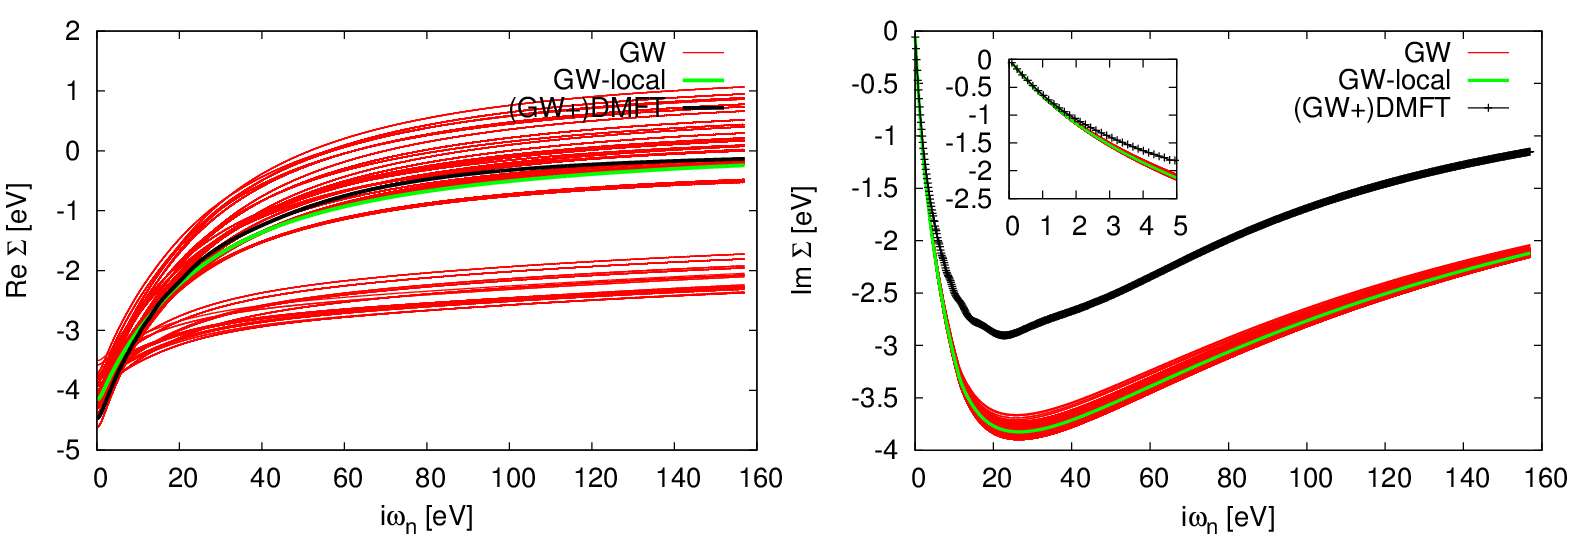
\includegraphics[width=1.0\textwidth]{figs/sigma_loc_compare.png}
\caption{The Selfenergy $\Sigma(i\omega_n)$ obtained from G$_0$W$_0$ (7x7x7 k-points)
 and GW+DMFT using the
G$_0$W$_0$ input for a $t_{2g}$-only model for SrVO$_3$ with $U(\omega)$ interaction determined
from cRPA.}
\label{fig:sigma_loc_compare}
\end{figure}

In Fig.\ref{fig:sigma_loc_compare} we show a comparison between the Selfenergy 
$\Sigma(i\omega_n)$ obtained from a G$_0$W$_0$ (7x7x7 k-points) calculation,
and GW+DMFT using the G$_0$W$_0$ input for a $t_{2g}$-only model for SrVO$_3$ with $U(\omega)$ interaction determined from cRPA.
The GW-local is the k-averaged part of the GW Selfenergy, and the GW+DMFT Selfenergy
is the local Selfenergy of the impurity model
after convergence of the GW+DMFT cycle including the non-local components
of the GW Selfenergy but subtracting the GW-local part as the doublecounting.
This means we have thrown away all contributions $G^{0,\mathrm{loc}}_{RR}W^{0,\mathrm{loc}}_{LRRL}$
arising from the interaction between the correlated subspace and the rest.

The discrepancy between the impurity Selfenergy and the k-averaged
GW Selfenergy, that can be seen especially in the imaginary part,
can then in principle have to reasons:

One contribution will be the contributions from the subspace
with the rest $G^{0,\mathrm{loc}}_{RR}W^{0,\mathrm{loc}}_{LRRL}$, as already discussed.
Another contribution can arise from the cRPA screening to obtain the effective
interaction $U(\omega)$. If the bare value is not the proper one, this would also
lead to a discrepancy especially in the tail sections of the Selfenergy, i.e.
if the value is too small, the tail will be smaller. 

\textbf{PLEASE NOTE:}
The GW doublecounting factor $\Sigma^{GW,DC}$ should not contain the Hartree
part, since the GW Selfenergy $\Sigma^{GW}_{XC}$ does not contain it.

\subsection{Possible problems with the DC}
One important factor is the causality of the different DC schemes.
The GW Selfenergy is causal and the impurity Selfenergy is causal,
but subtracting a DC term can make the combined Selfenergy noncausal
\begin{align}
\Sigma^{GW+DMFT} &= \Sigma^{GW,loc} - \Sigma^{DC} + \Sigma^{imp}.
\end{align}
It only comes down to personal preference, whether the DC should be understood
as taking out contibutions from GW, so that GW is a correction to DMFT
\begin{align}
\Sigma^{GW+DMFT} &=  \Sigma^{imp} + \left(\Sigma^{GW,loc} - \Sigma^{DC}\right) ,
\end{align}
or whether one takes out contibutions from DMFT, so that DMFT is a correction to GW
\begin{align}
\Sigma^{GW+DMFT} &=  \Sigma^{GW,loc} + \left(\Sigma^{imp} - \Sigma^{DC}\right) .
\end{align}



\subsection{High-frequency correction for $G_{loc}W_{loc}$}
When evaluating the doublecounting factor
\begin{align}
\Sigma^{GW,DC} &= -G^{0,\mathrm{loc},L}W^{0,\mathrm{loc},L},
\end{align}
on the Matsubara axis (it should be calculated directly in the GW code instead),
we have to correct the frequency sum (orbital indices are suppressed)
\begin{align}
\Sigma^{GW,DC}(i\omega_n) 
&= -\frac{1}{\beta} \sum_{i\nu_n} G^{0,\mathrm{loc}}(i\omega_n - i\nu_n )
                                        W^{0,\mathrm{loc}}(i\nu_n),
\end{align}
where $i\omega_n$ is a fermionic and $i\nu_n$ is a bosonic Matsubara
frequency. 
Rewriting the sum (and suppressing the 0,loc lables)
by using $W(i\nu_n) = W(-i\nu_n) \in \mathbb{R}$ we get
\begin{align}
\Sigma^{GW,DC}(i\omega_n) 
&= -\frac{1}{\beta} \sum_{i\nu_n} G(i\omega_n - i\nu_n)
                                  W(i\nu_n)\\
%
&= -\frac{1}{\beta} G(i\omega_n)W(0)
-\frac{1}{\beta} \sum_{n=1}^{\infty} \left[ G(i\omega_n+i\nu_n)+G(i\omega_n-i\nu_n)\right]
                                        W(i\nu_n).
%
\end{align}
We seperate out the $n=0$ term since the high-frequency
correction for the bosonic $W(inu_n)$ would diverge at $n=0$.

The second term has to be corrected, where we will use corrections up to second order,
i.e.
\begin{align}
& -\frac{1}{\beta} \sum_{n=1}^{\infty} \left[ G(i\omega_n+i\nu_n)+G(i\omega_n-i\nu_n)\right]
                                        W(i\nu_n) \\
%
&= -\frac{1}{\beta} \sum_{n=1}^{\infty} 
\left[ \left(G(i\omega_n+i\nu_n)+G(i\omega_n-i\nu_n) 
       -\frac{1}{i\omega_n+i\nu_n}-\frac{1}{i\omega_n-i\nu_n}
       -\frac{g_2}{(i\omega_n+i\nu_n)^2}-\frac{g_2}{(i\omega_n-i\nu_n)^2} \right)
\right. \\
%
& \hspace{7.2cm} \left.
+\left(\frac{1}{i\omega_n+i\nu_n}+\frac{1}{i\omega_n-i\nu_n}
       +\frac{g_2}{(i\omega_n+i\nu_n)^2}+\frac{g_2}{(i\omega_n-i\nu_n)^2} \right)
       \right] \\
%
%
& \hspace{2cm} \times \left[
\left(W(i\nu_n) - w_0 - \frac{w_2}{(i\nu_n)^2}\right) 
+ \left( w_0 + \frac{w_2}{(i\nu_n)^2} \right)
\right]
\end{align}
We have to be careful about the shift in the denominator since
for large $\nu_n$ 
\begin{align}
\frac{1}{i\omega_n + i\nu_n} &\sim \frac{1}{i\nu_n} \\
%
\frac{1}{(i\omega_n + i\nu_n)^2} 
&= \frac{1}{-\omega_n^2 -\nu_n^2 - 2\nu_n\omega_n} \sim -\frac{1}{2\omega_n\nu_n}
%
\end{align}
So even the second order in the Green's function only decays as $1/\nu_n$
in the frequency sum.
Therefore, it might be better to put the frequency shift in $W(i\nu)$,
since the decay is faster with $1/\nu_n^2$.
I tried to derive this but somehow failed to 
evaluate the terms analytically (see commented out section in tex file)
% 
% So rewriting the sum we get 
% \begin{align}
% \Sigma^{GW,DC}(i\omega_n) 
% &= -\frac{1}{\beta} \sum_{i\nu_n} G(i\omega_n+i\nu_n)
%                                   W(i\nu_n)\\
% %
% &= -\frac{1}{\beta} \sum_{ix_n} G(ix_n)
%                                   W(ix_n - i\omega_n) \\
% %
% &= -\frac{1}{\beta} \sum_{n=0}^{\infty}
% \left[ G(ix_n)W(i\omega_n-ix_n) 
%     + G^*(ix_n)W(i\omega_n+ix_n)
% \right]
% \end{align}
% where $ix_n$ is a fermionic Matsubara frequency. Correcting up to
% second order we get
% \begin{align}
% &-\frac{1}{\beta} \sum_{n=0}^{\infty}
% \left[ G(ix_n)W(i\omega_n-ix_n) 
%     + G^*(ix_n)W(i\omega_n+ix_n) 
% \right]\\
% %
% =&-\frac{1}{\beta} \sum_{n=0}^{\infty}
% \left[ \mathrm{Re}G(ix_n)\left( W(i\omega_n-ix_n) + W(i\omega_n+ix_n) \right) \right.\nonumber \\
%  & \left. \hspace{1.35cm}   +\mathrm{Im}G(ix_n)\left( W(i\omega_n-ix_n) - W(i\omega_n+ix_n) \right)
% \right]\\
% %
% %
% =&-\frac{1}{\beta} \sum_{n=0}^{\infty}
% \left[ \left(\mathrm{Re}G(ix_n) - \frac{g_2}{(ix_n)^2} + \frac{g_2}{(ix_n)^2}\right) \right. \nonumber \\
% %
% & \times \left( W(i\omega_n-ix_n) + W(i\omega_n+ix_n) 
%  - 2w_0-\frac{w_2}{(i\omega_n-ix_n)^2} -\frac{w_2}{(i\omega_n+ix_n)^2} \right.\nonumber  \\
% &\left. \hspace{6.3cm}  + 2w_0+\frac{w_2}{(i\omega_n-ix_n)^2}+\frac{w_2}{(i\omega_n-ix_n)^2}\right) \nonumber \\
% %
% %
% %
% &\hspace{1.5cm} +\left(\mathrm{Im}G(ix_n) - \frac{1}{ix_n} + \frac{1}{ix_n}\right) \nonumber \\
% %
% & \times \left( W(i\omega_n-ix_n) - W(i\omega_n+ix_n) 
%  -\frac{w_2}{(i\omega_n-ix_n)^2} +\frac{w_2}{(i\omega_n+ix_n)^2} \right. \nonumber \\
% &\left. \hspace{6.3cm}  + \frac{w_2}{(i\omega_n-ix_n)^2}-\frac{w_2}{(i\omega_n-ix_n)^2}\right)
% \end{align}
% 
% ASD
% ASd
% ASD
% ASd
% 
% \begin{align}
% &-\frac{1}{\beta} \sum_{n=0}^{\infty}
% \left[ G(ix_n)W(i\omega_n-ix_n) 
%     + G^*(ix_n)W(i\omega_n+ix_n) 
% \right]\\
% %
% =&-\frac{1}{\beta} \sum_{n=0}^{\infty}
% s
% \end{align}

Expanding the 


%%%%%%%%%%%%%%%%%%%%%%%%%%%%%%%%%%%%%%%%%%%%%%%%%%%%%%%%%%%%%%%%%%%%%%%%%%%%%%%%%%%%%%%%%%%%%%%%
%%%%%%%%%%%%%%%%%%%%%%%%%%%%%%%%%%%%%%%%%%%%%%%%%%%%%%%%%%%%%%%%%%%%%%%%%%%%%%%%%%%%%%%%%%%%%%%%
%%%%%%%%%%%%%%%%%%%%%%%%%%%%%%%%%%%%%%%%%%%%%%%%%%%%%%%%%%%%%%%%%%%%%%%%%%%%%%%%%%%%%%%%%%%%%%%%

\section{Product basis}
In the GW formalism we encounter objects such as the inverse dielectric function
\begin{align}
 \epsilon^{-1},
\end{align}
which is a two-particle operator. The standard way to specify the action of a two-particle operator
is to start from a complete orthonormal single-particle basis $\{ \ket{i} \}$, where
\begin{align}
 \braket{\vec{r} | i} &= \psi_i(\vec{r}),
\end{align}
with a complex valued function $\psi_i: R^3\rightarrow \mathbb{C}$.
Then one introduces a two-particle basis $\{ \ket{ij} \}$, which is composed of the single-particle states via
\begin{align}
\braket{\vec{r}\vec{r}' | ij} 
&= \Big( \bra{\vec{r}} \otimes \bra{\vec{r}'} \Big) \Big( \ket{i} \otimes \ket{j} \Big) \\
&= \psi_i(\vec{r})\psi_j(\vec{r}').
\end{align}
In this basis, any two-particle operator $A$ can be represented as a rank-4 tensor
by its action on the two-particle basis states
\begin{align}
A_{ijkl} &= \braket{ij | A | kl }  \\
&= \int \int \mathrm{d}\vec{r}\mathrm{d}\vec{r}' \, \psi^*_i(\vec{r})\psi^*_j(\vec{r}') 
                                          A(\vec{r},\vec{r}') \psi_l(\vec{r}')\psi_k(\vec{r}),
\end{align}
where we have assumed that 
\begin{align}
 \braket{\vec{r}\vec{r}' | A | \vec{r}''\vec{r}''' }
 &= A(\vec{r},\vec{r}') \delta(\vec{r}-\vec{r}'') \delta(\vec{r}'-\vec{r}'''),
\end{align}
which applies to the Coulomb interaction operator and all other operators we will consider here.

Our goal is to obtain a matrix (rank-2) representation of the two-particle operator $A$, so that we can 
define a proper inverse $A^{-1}$ or a multiplication $AB$ between these operators. 
This is usually done in two ways:

%%%%%%%%%%%%%%%%%%%%%%%%%%%%%%%%%%%%%%%%%%%%%%%%%%%%%%%%%%%%%%%%%%%%%%%%%%%%%
\subsection{Index combination}
In the two-particle basis the structure of the Tensor-elements
\begin{align}
 A_{ijkl} &= \braket{ij | A | kl } ,
\end{align}
suggests that we could also interpret each basis state as
\begin{align}
 \ket{a} := \ket{ ij } &= \ket{i}\otimes \ket{j} ,
\end{align}
with a single basis state $\ket{a}$, where the index $a$ now runs over $N^2$ values
if we have $N$ single particle states $\ket{i}$. In this notation, we can indeed write the tensor elements
as matrix elements
\begin{align}
 A_{ab} &= \braket{a | A | b } \\
 &= \braket{ij | A | kl }   \\
  &= A_{(ij)(kl)} .
\end{align}

\subsubsection{Properties and consistency}

The combination of the two left, the ``outgoing'' indices $ij$ and the right, the ``incoming'' $kl$ is in principle arbitrary.
We could also combine the indices $ik$ of the first partcile and $jl$ of the second particle. 
Though, the $(ij)(kl)$ combination should be preferrable, since it does not mix vectors $\ket{i}$ with their
dual counterpart $\bra{i}$. 

Furthermore, in cases where we want to apply this scheme, the tensor operations can indeed be rewritten
as a matrix multiplication in the combined ``ingoing-outgoing'' index notation. For example
the screened interaction $W$ is given by
\begin{align}
W_{ijkl} &= [ v + vPW ]_{ijkl} \\
&= v_{ijkl} + \sum_{mnop} v_{ijmn}P_{mnop}W_{opkl},
\end{align}
with the bare interaction $v$ and the polarization $P$. Using the combined index notation we get the representation
\begin{align}
W_{ab} &= W_{(ij)(kl)} \\
&= v_{(ij)(kl)} + \sum_{(mn)(op)} v_{(ij)(mn)}P_{(mn)(op)}W_{(op)(kl)} \\
&= v_{ab} + \sum_{cd} v_{ac}P_{cd}W_{da} \\
&= [v + vPW]_{ab},
\end{align}
where $vPW$ is to be understood as the matrix product of $v,P$ and $W$ in the combined index notation.

\subsubsection{Tensor inverse}

Now let us try to obtain a closed expression of $W$ satisfying this expression, which
is not possible in the 4-index tensor notation.
For this, we need to define first an object $\unity$ that serves as the identity element, which then will
allow us to poperly define an inverse of a matrix in the combined index notation.
The identity element should have the following property
\begin{align}
 \unity A &= A =  A \unity ,
\end{align}
where $A$ is a two-particle tensor, which means
\begin{align}
A_{(ij)(kl)} &= A_{ab} \\
&= [\unity A]_{ab} \\
&= \sum_c \unity_{ac} A_{ca} \\
&= \sum_{mn} \unity_{(ij)(mn)} A_{(mn)(kl)} .
\end{align}
From this we conclude that 
\begin{align}
 \unity_{(ij)(mn)} &= \delta_{im}\delta_{jn} \\
 \Rightarrow \unity_{ac} &= \delta_{ac},
\end{align}
which leads to the natural definition of the identity element in the combined index notation.
It can be directly seen that also $ A \unity = A$ is fulfilled.

From this we can define the inverse $A^{-1}$ as the standard matrix inverse in the combined index notation
that fulfills
\begin{align}
A^{-1}A &= AA^{-1} = \unity,
\end{align}
since
\begin{align}
[A^{-1}A]_{(ij)(kl)} &= [A^{-1}A]_{ab} \\
&= \delta_{ab} \\
&= \delta_{ik}\delta_{kl} \\
&= \unity_{(ij)(kl)}
\end{align}
With this, we can finally solve the equation above for the screened interaction
\begin{align}
 W &= v + vPW \\
 \Rightarrow (\unity - vP) W &= v \\
 \Rightarrow  W &=(\unity - vP)^{-1} v ,
\end{align}
By contruction, the tensor elements $W_{ijkl} =[(\unity - vP)^{-1} v]_{ijkl}$
will now satisfy the equation above for the screened interaction.

\subsubsection{Problems}
Possible problems are:
\begin{itemize}
\item A two-particle operator diagonal in position representation cannot be inverted
in the combined index-notation! This can be for example a purely local Coulomb interaction!

Consider 
\begin{align}
 \braket{\vec{r}\vec{r}' | A | \vec{r}''\vec{r}''' }
 &= A(\vec{r}) \delta(\vec{r}-\vec{r}') \delta(\vec{r}-\vec{r}'') \delta(\vec{r}'-\vec{r}'''),
\end{align}
and we assume that $A(\vec{r})=a>0$ constant, \textit{i.e.} it does not matter where the particles interact.
As long as their positions are identical they pick up a factor $a$.

This leads to the following tensor elements
\begin{align}
A_{ijkl} &= \braket{ij | A | kl }  \\
&= \int \int \mathrm{d}\vec{r}\mathrm{d}\vec{r}' \, \psi^*_i(\vec{r})\psi^*_j(\vec{r}') 
                                          a \delta(\vec{r}-\vec{r}') \psi_l(\vec{r}')\psi_k(\vec{r}) \\
&=a  \int \mathrm{d}\vec{r} \, \psi^*_i(\vec{r})\psi^*_j(\vec{r}) 
                                          \psi_l(\vec{r})\psi_k(\vec{r}) .
\end{align}
For the case of real wave functions we see that we always get a non-zero contribution when we pair 
two indices with one another, leading to an integral of the form
\begin{align}
a  \int \mathrm{d}\vec{r} \, \psi^2_m(\vec{r}) \psi^2_n(\vec{r}) \neq 0
\end{align}
For the example of $N=2$ single-particle states $\psi_i(\vec{r})$, we can choose two out of four indices to pair, then
the last one has to be paired with $N=2$ choices for the index, leading to 8 combinations which are at least non-zero.
In the combined index notation we then can arrive at the following matrix 
(\cng{Note: I have confirmed this numerically for a few basis sets})
\begin{align}
 A &= a
 \begin{pmatrix}
  c_1 & 0 & 0 & c_3 \\
  0   & c_2 & c_2 & 0 \\
  0 & c_2 & c_2 & 0 \\
  c_3 & 0 & 0 & c_4 
 \end{pmatrix},
\end{align}
where we can immediately see that this matrix cannot be inverted since two columns are linearly dependent (even identical).

\item A ``constant'' operator $A(\vec{r},\vec{r}')=c\neq 0$  can be inverted! (See discussion in next section)

\end{itemize}


%%%%%%%%%%%%%%%%%%%%%%%%%%%%%%%%%%%%%%%%%%%%%%%%%%%%%%%%%%%%%%%%%%%%%%%%%%%%%

\subsection{Aryasetiawan-style}
\subsubsection{Defining the new basis set}
We start by rewriting the equation for the tensor elements in the two-particle basis in the 
following way 
\begin{align}
 \braket{ij | A | kl }  
&= \int \int \mathrm{d}\vec{r}\mathrm{d}\vec{r}' \, \psi^*_i(\vec{r})\psi^*_j(\vec{r}') 
                                          A(\vec{r},\vec{r}') \psi_l(\vec{r}')\psi_k(\vec{r}) \\
%
&= \int \int \mathrm{d}\vec{r}\mathrm{d}\vec{r}' \, \psi^*_i(\vec{r})\psi_k(\vec{r}) 
                                          A(\vec{r},\vec{r}') \psi^*_j(\vec{r}')\psi_l(\vec{r}') \\
%
&= \int \int \mathrm{d}\vec{r}\mathrm{d}\vec{r}' \, \underbrace{ \Big( \psi^*_k(\vec{r}) \psi_i(\vec{r}) \Big)^* }_{B^*_a(\vec{r})}
                                          A(\vec{r},\vec{r}') \underbrace{ \psi^*_j(\vec{r}')\psi_l(\vec{r}') }_{B_b(\vec{r}' )} \\
&= \braket{ B_a | A | B_b } .
\end{align}
From these observation we see that we should define new basis states $\{ B_a \}$ by the product of the single-particle
states by
\begin{align}
 \braket{ \vec{r} | B_a } := \psi^*_i(\vec{r}) \psi_j(\vec{r}),
\end{align}
where the index $a:=a(i,j)$ lables the combination of the indices $i,j$. As a result, for a finite number of single-particle
states $N=\mathrm{dim}\{ \ket{i} \}$, we have $N^2$ new basis states $\{ B_a \}$, and could define the relation between the indices
as
\begin{align}
 a(i,j) := iN + j.
\end{align}
Though, the new set $\{ B_a \}$ is \textit{not} a basis, since it is overcomplete/linearly dependent and in addition not orthonormal.
For example if there exist at least two real single-particle basis functions $\psi_i,\psi_j$, one has 
\begin{align}
\psi_i(\vec{r})\psi_j(\vec{r}) = B_a(\vec{r}) = B_b(\vec{r}) = \psi_j(\vec{r})\psi_i(\vec{r}),
\end{align}
where $a\neq b$.
Also, for a states with indices $a(i,i)$ and $b(i,i)$, which leads to
\begin{align}
 \braket{B_a | B_b} &= \int \mathrm{d}\vec{r} \, \psi^*_i(\vec{r}) \psi_i(\vec{r}) \psi^*_j(\vec{r}) \psi_j(\vec{r}) \\
 &= \int \mathrm{d}\vec{r} \, |\psi_i(\vec{r})|^2 |\psi_j(\vec{r})|^2 
\end{align}
which is usually larger than zero for $a\neq b$, i.e. $i=j$ and not equal to $1$ in case $a=b$, i.e. $i\neq j$.

The overlap matrix for the new set $\{ B_a \}$ is therefore different from the unit matrix.
If we define 
\begin{align}
 v := 
 \begin{pmatrix}
%   \ket{B_1}\\ \ket{B_2}\\\ket{B_3}\\ \vdots \\ \ket{B_{N^2}}
\ket{B_1} & \ket{B_2} & \ket{B_3}& \cdots & \ket{B_{N^2}}  
 \end{pmatrix},
\end{align}
then the overlap matrix can be written as
\begin{align}
O &= v^{\dagger}\cdot v,
\end{align}
since
\begin{align}
O_{ab} &= (v^{\dagger}\cdot v)_{ab} \\
 &= \braket{B_a | B_b} .
\end{align}
Due to the overcompleteness, some columns of $O$ will not be linear independent, i.e. some of the Eigenvalues 
$\lambda_i$ of $O$ will be equal to zero.

\subsubsection{Reduction of the basis set and reorthonormalization}

After diagonalizing $O$ to obtain the Eigenvectors $o_1,o_2,...,o_{N^2}$, we throw away the ones with Eigenvalue zero 
and set up the matrices
\begin{align}
 U &=
 \begin{pmatrix}
  o_1 & o_2 & o_3 & \cdots o_{N_r}
 \end{pmatrix} \in \mathbb{C}^{N^2 \times N_r},
\end{align}
where $N_r \leq N^2$ is the number of Eigevectors with nonzero Eigenvalue,
and
\begin{align}
 D^{-1/2} &:= \mathrm{diag}( {\lambda_1}^{-1/2}, \ {\lambda_2}^{-1/2}, \ {\lambda_3}^{-1/2}, \ \cdots,\ {\lambda_{N_r}}^{-1/2}  ) 
 \in \mathbb{R}^{N_r \times N_r},
\end{align}
where $\lambda_i$ are the nonzero Eigenvalues of $O$.


The elements of the following vector
\begin{align}
\tilde{v} := vUD^{-1/2} ,
\end{align}
will then yield a new set of $N_r$ basis functions which are complete and orthonormal, as can be seen from
the new overlap matrix
\begin{align}
\tilde{O} &= \tilde{v}^{\dagger}\cdot \tilde{v} \\
&= D^{-1/2}U^{\dagger} (v^{\dagger} \cdot v) UD^{-1/2} \\
&= D^{-1/2} \underbrace{U^{\dagger} O U}_{=D} D^{-1/2} \\
&= \unity  \in \mathbb{R}^{N_r \times N_r}.
\end{align}

\textit{Remark:}
To reduce the size of the basis for computational efficiency, one can also exclude Eigenvectors with a finite, 
but small Eigenvalue, i.e. below some treshhold $\delta > \lambda_i$.
Then the new basis will only be approximately complete and orthonormal, but the error can be controlled by choosing
$\delta$ sufficiently small.

\subsubsection{Product basis matrix elements}

After having obtained the new complete orthonormal basis $\{ \tilde{B}_a  \}$, the matrix elements
of any two-particle operator are then given as
\begin{align}
A_{ab}
&= \braket{ \tilde{B}_a | A | \tilde{B}_b } \\
&= \int \int \mathrm{d}\vec{r}\mathrm{d}\vec{r}' \,  \tilde{B}^*_a(\vec{r})  A(\vec{r},\vec{r}') \tilde{B}_b(\vec{r}').
\end{align}
The representation of $A$ in the product basis is then given as
\begin{align}
A &= \sum_{a,b} \ket{\tilde{B}_a}A_{ab}\bra{\tilde{B}_b} .
\end{align}
or in the position representation \cng{DOES THIS MAKE SENSE?}
\begin{align}
 A(\vec{r},\vec{r}') &= \sum_{a,b} \braket{\vec{r}|\tilde{B}_a} A_{ab}\braket{\tilde{B}_b|\vec{r}'} \\
 &= \sum_{a,b} \tilde{B}_a(\vec{r}) A_{ab}\tilde{B}^*_b(\vec{r}') .
\end{align}
\cng{CHECK HERE IF BOTH REPRESENTATIONS LEAD TO THE SAME RESULT!!! The product basis should recover
the right A(r-r'), shouldn't it? (I think so...) Can we actually prove this?}


\subsubsection{Switching between the product and the two-particle basis}
If we want to obtain the original tensor representation of a two-particle operator in the 
product basis, we have to evaluate \cng{DOES THIS MAKE SENSE?}
\begin{align}
A_{ijkl} &= \braket{ij | A | kl }  \\
&= \int \int \mathrm{d}\vec{r}\mathrm{d}\vec{r}' \, \psi^*_i(\vec{r})\psi^*_j(\vec{r}') 
                                          A(\vec{r},\vec{r}') \psi_l(\vec{r}')\psi_k(\vec{r}) \\
&= \sum_{a,b}\int \int \mathrm{d}\vec{r}\mathrm{d}\vec{r}' \, \psi^*_i(\vec{r})\psi^*_j(\vec{r}') 
         \tilde{B}_a(\vec{r}) A_{ab}\tilde{B}^*_b(\vec{r}') \psi_l(\vec{r}')\psi_k(\vec{r}).
\end{align}
The other way round, if we have a two-particle operator given in the two-particle basis, the product basis
representation can be obtained by
\begin{align}
A_{ab}
&= \braket{ \tilde{B}_a | A | \tilde{B}_b } \\
&= \int \int \mathrm{d}\vec{r}\mathrm{d}\vec{r}' \,  \tilde{B}^*_a(\vec{r})  A(\vec{r},\vec{r}') \tilde{B}_b(\vec{r}') \\
&=\sum_{ijkl} \int \int \mathrm{d}\vec{r}\mathrm{d}\vec{r}' \,  \tilde{B}^*_a(\vec{r})  
    \psi_i(\vec{r})\psi_j(\vec{r}') A_{ijkl} \psi^*_l(\vec{r}')\psi^*_k(\vec{r}) \tilde{B}_b(\vec{r}') .
\end{align}


% \begin{align}
%  \braket{ii | A | jj }  
% &= \int \int \mathrm{d}\vec{r}\mathrm{d}\vec{r}' \, \psi^*_i(\vec{r})\psi_j(\vec{r}) 
%                                           A(\vec{r},\vec{r}') \psi^*_i(\vec{r}')\psi_j(\vec{r}')
% \end{align}
% 
% \begin{align}
%  \braket{ij | A | ij }  
% &= \int \int \mathrm{d}\vec{r}\mathrm{d}\vec{r}' \, \psi^*_i(\vec{r})\psi_i(\vec{r}) 
%                                           A(\vec{r},\vec{r}') \psi^*_j(\vec{r}')\psi_j(\vec{r}')
% \end{align}
% 
% \begin{align}
%  \braket{ij | A | ji }  
% &= \int \int \mathrm{d}\vec{r}\mathrm{d}\vec{r}' \, \psi^*_i(\vec{r})\psi_j(\vec{r}) 
%                                           A(\vec{r},\vec{r}') \psi^*_j(\vec{r}')\psi_i(\vec{r}')
% \end{align}

\subsubsection{Tensor inverse}

Since in the product basis any two-particle operator can now be
represented as a matrix/rank-2 tensor, we can finally define its inverse $\tilde{A}^{-1}$ as the standard Matrix inverse, which then in the product basis fulfils the property
\begin{align}
 (\tilde{A}^{-1}A)_{ab}
&= \braket{ \tilde{B}_a | \tilde{A}^{-1}A | \tilde{B}_b } \\
&= \delta_{ab}.
\end{align}
In the position representation
\begin{align}
\braket{\vec{r} | \tilde{A}^{-1}A | \vec{r}' }
 &= \sum_{a,b} \braket{\vec{r}|\tilde{B}_a} (\tilde{A}^{-1}A)_{ab}\braket{\tilde{B}_b|\vec{r}'} \\
%
&= \sum_{a,b} \braket{\vec{r}|\tilde{B}_a} \delta_{ab} \braket{\tilde{B}_b|\vec{r}'} \\
&= \sum_{a} \braket{\vec{r}|\tilde{B}_a} \braket{\tilde{B}_a|\vec{r}'} \\
&= \braket{\vec{r}|\vec{r}'} \\
&= \delta(\vec{r}-\vec{r}'),
\end{align}
if the product basis is complete.

%\braket{\vec{r}|\tilde{B}_a} A_{a\braket{\tilde{B}_b|\vec{r}'}

\subsubsection{Problems}
Possible problems are:
\begin{itemize}
 \item A ``constant'' tensor of the form $A(\vec{r},\vec{r}')=c\neq 0$ cannot be inverted! 
 \cng{I'm not sure, this is maybe correct behaviour?}

 Let us assume we obtain a final basis state $\ket{\tilde{B}_o}$ in a one-dimensional system
 which is a real odd function in position representation, \textit{i.e.}
 \begin{align}
  \tilde{B}_o(r) &= -\tilde{B}_o(-r).
 \end{align}
For a constant tensor this leads to the following
 \begin{align}
A_{ab}
&=c \int \int \mathrm{d}\vec{r}\mathrm{d}\vec{r}' \,  \tilde{B}^*_a(\vec{r})  \tilde{B}_b(\vec{r}') \\
&=c \left(\int \mathrm{d}\vec{r} \, \tilde{B}^*_a(\vec{r}) \right) \left( \int \mathrm{d}\vec{r}'\,  \tilde{B}_b(\vec{r}'), \right),   
\end{align}
\textit{i.e.} the two integrations over the basis states decouple, and everytime $a$ or $b$ is equal to the
real odd function $\tilde{B}_o$, we obtain zero. Therefore, the $o$-th column and row is equal to zero.
Which means, we have at least one Eigenvalue equal to zero and, therefore, the tensor
in the product basis cannot be inverted.

\item The ``identity'' tensor of the form $\braket{ij|A|kl}=\delta_{ik}\delta_{jl}$ 
cannot be inverted! 
This can be seen from
\begin{align}
A_{ab}
&= \braket{ \tilde{B}_a | A | \tilde{B}_b } \\
&=\sum_{ijkl} \int \int \mathrm{d}\vec{r}\mathrm{d}\vec{r}' \,  \tilde{B}^*_a(\vec{r})  
    \psi_i(\vec{r})\psi_j(\vec{r}') A_{ijkl} \psi^*_l(\vec{r}')\psi^*_k(\vec{r}) \tilde{B}_b(\vec{r}') \\
 &=\sum_{ij} \int \int \mathrm{d}\vec{r}\mathrm{d}\vec{r}' \,  \tilde{B}^*_a(\vec{r})  
 \psi_i(\vec{r})\psi_j(\vec{r}') \psi^*_j(\vec{r}')\psi^*_i(\vec{r}) \tilde{B}_b(\vec{r}') \\
  &=\sum_{ij} \left(\int \mathrm{d}\vec{r} \,  \tilde{B}^*_a(\vec{r})  
 |\psi_i(\vec{r})|^2 \right)
 \left(\int \mathrm{d}\vec{r}' \,  \tilde{B}_b(\vec{r}')  
 |\psi_j(\vec{r}')|^2 \right).
\end{align}
 If one basis function $\tilde{B}_a(\vec{r})$ is an odd function, 
 the full column $a$ and row $a$ will be zero, so 
 we have at least one Eigenvalue equal to zero and, therefore, the tensor
in the product basis cannot be inverted.
\end{itemize}



%%%%%%%%%%%%%%%%%%%%%%%%%%%%%%%%%%%%%%%%%%%%%%%%%%%%%%%%%%%%%%%%%%%%%%%%%%%%%%%%%%%%%%%%%%%%%%%%
%%%%%%%%%%%%%%%%%%%%%%%%%%%%%%%%%%%%%%%%%%%%%%%%%%%%%%%%%%%%%%%%%%%%%%%%%%%%%%%%%%%%%%%%%%%%%%%%
%%%%%%%%%%%%%%%%%%%%%%%%%%%%%%%%%%%%%%%%%%%%%%%%%%%%%%%%%%%%%%%%%%%%%%%%%%%%%%%%%%%%%%%%%%%%%%%%


\section{The GW part}

On the basis of $H^{DFT}$ a $G_0W_0$ calculation has to be performed on the full
system. By this, the Selfenergy in the Kohn-Sham basis is obtained for all states
\begin{align}
 \Sigma_{\nu\nu'}(k,\omega)
 &= \left[ G_0W_0  \right]_{\nu\nu'}(k,\omega).
\end{align}
By this, the GW estimate for the full interacting {\GF} is given by
\begin{align}
 G^{GW}_{\nu\nu'}(k,\omega) 
 &= \left[ \unity(\omega +\mu +i\delta) -H^{DFT}(k)+v^{XC}(k) - \Sigma^{GW}(k,\omega)  \right]^{-1}_{\nu\nu'}.
\end{align}


\subsection{Output for DMFT}
At this point the basis transformation to the local Wannier basis will be
performed on the GW side.
For the next step of the DMFT calculation one needs
on a mesh in k-space in the full Brillouin zone:
\begin{itemize}
\item $\beta$: The inverse temperature used for defining $\omega_n=(2n+1)\pi/\beta$.
\item $\epsilon_m(k)$: The eigenvalues  of $H^{DFT}(k)$ in the Wannier basis
for all relevant orbitals
\item $\mu$: The chemical potential that yields the correct physical number of electrons $N_e$. It is not needed if all $\epsilon_m(k)$ are given 
with respect to the Fermi level.
for $H^{DFT}$
\item $v^{XC}_{mm'}(k)$: The value of the exchange-correlation potential 
in the Wannier basis for all relevant orbitals
\item $\Sigma^{GW,XC}_{mm'}(k,i\omega)$: The exchange-correlation 
Selfenergy within GW in the Wannier basis for all relevant orbitals on imaginary frequencies $\omega$.
\item $\Sigma^{GW,imp,XC}_{mm'}(i\omega) = -[G^{0,loc,L}W^{0,loc,L}]^{XC}_{mm'}$
The exchange-correlation selfenergy of the impurity model solved in GW, \textit{i.e.}
all indices and internal transitions restricted to the correlated subspace
\item $V_{abcd}(q)$: The bare Coulomb interaction elements in the Wannier basis for all relevant orbitals.
\cng{?Do we have V in the product basis of the 3d orbitals? When do we construct this? IMPORTANT: IS the spin also incorporated or kept separate?}
\item $P^{GW}_{abcd}(q,i\nu)$: The polarization  in the Wannier basis for all relevant orbitals on imaginary frequencies.\cng{?Do we have P in the product basis of the 3d orbitals? When do we construct this?}
\item $P^{GW,imp}_{abcd}(i\nu) = [G^{0,loc,L}G^{0,loc,L}]_{abcd}$
The polarization of the impurity model solved in GW, \textit{i.e.}
all indices and internal transitions restricted to the correlated subspace
\end{itemize}
{\it All output from the GW calculation will be in atomic units and
has to be converted to eV!!}


\section{The DMFT part}

Within DMFT we then calculate a local correction $\Sigma^{DMFT}$ for a subset of correlated
Wannier orbitals.

The input of the calculation will be the output of the GW calculation. First, one will usually apply a Wannier-interpolation of the GW data to obtain a fine k-mesh
since the GW output will be given on a very coarse grid.

\subsection{The self-consistency cycle}

We then proceed as follows:

\begin{enumerate}

%\item Transform the Selfenergy from GW to the imaginary Matsubara axis by
%\begin{align}
%\Sigma^{GW}_{mm'}(k,i\omega_n)
%&= \frac{1}{2\pi i} \int \, \frac{\Sigma^{GW}_{mm'}(k,\omega)}{\omega - i\omega_n}\ \mathrm{d}\omega , \mbox{\hspace{1cm} or}\\
%&= \frac{1}{\pi} \int \, \frac{\mathrm{Im}[\Sigma^{GW}_{mm'}(k,\omega)]}{\omega - i\omega_n} \ \mathrm{d}\omega , \mbox{\hspace{0.7cm} or} \\
%&= \frac{1}{\pi i} \int \, \frac{\mathrm{Re}[\Sigma^{GW}_{mm'}(k,\omega)]}{\omega - i\omega_n} \ \mathrm{d}\omega .
%\end{align}

%\item Calculate the local diagonal part of the GW Selfenergy ONLY for the correlated subset of orbitals $f$ that will be later replaced by the DMFT result
%\begin{align}
% \Sigma^{GW,loc}_{f}(i\omega_n)
% &= \frac{1}{N_k}\sum_k \Sigma^{GW}_{ff}(k,i\omega_n).
%\end{align}


%\item (This step can be omitted if the correct physical number of electrons $N_e$ is already known)
% 
%Construct the initial non-interacting {\GF} on the imaginary Matsubara axis via
%\begin{align}
%   G_{0,mm'}(k,i\omega_n) 
% &= \left[ \unity(i\omega_n +\mu) -H^{DFT}(k)   \right]^{-1}_{mm''},
%\end{align}
% and calculate the total number of electrons
%\begin{align}
%  N_e
% &= \lim_{\tau\rightarrow 0^-} \frac{1}{\beta N_k} 
%                \sum_{i\omega_n}\sum_{k,m}G_{0,mm}(k,i\omega_n) \mathrm{e}^{-i\omega_n\tau}.
%\end{align}

\item Make a first guess for the local DMFT impurity Selfenergy  $\Sigma^{imp}$ and polarization $P^{imp}$, for example one can use the GW result
\begin{align}
\Sigma^{imp}(i\omega_n) &=  \Sigma^{GW,imp,XC}(i\omega_n) + \Sigma^{imp,Hartree} \\
P^{imp}(i\nu_n) &=  P_{GW,imp}(i\nu_n) .
\end{align}
Please note that $\Sigma$ is a matrix in the orbital basis $\Sigma_{mm'}$ and $P$ is a tensor
$P_{\alpha\beta}$ in the product basis $\{ B_{\alpha} \}$, where $P,V$ and all further tensors are
treated as standard matrices
$P_{\alpha\beta} = \braket{ B_{\alpha} | P | B_{\beta} }$, etc.

\item Set up the interacting {\GF} $G$ and the screened interaction $W$, where the impurity component of the GW contribution for the correlated orbitals is replaced by the DMFT contribution.
%In the first step when using $\Sigma^{imp}_{ff} =  \Sigma^{GW,loc}_{f}$ this 
%term is zero.
\begin{align}
 G(k,i\omega_n) 
 &= \left[ \unity(i\omega_n+\mu ) -H^{DFT}(k) + v^{XC}(k) + \Sigma^{Hartree}_{DFT} \right.\\
          & \hspace{1cm}- \Sigma^{XC}_{GW}(k,i\omega_n) 
          + \Sigma_{GW,imp}^{XC}(i\omega_n)
          \left. - \Sigma_{imp}(i\omega_n)
           \right]^{-1} \\
%
W(q,i\nu_n) &= \left[ V^{-1}(q) - P_{GW}(q,i\nu_n) + P_{GW,imp}(i\nu_n) 
                              -P_{imp}(i\nu_n)\right]^{-1}
\end{align}
Adjust the chemical potential $\mu$ in a way such that the desired
filling
\begin{align}
  N_e
 &= \lim_{\tau\rightarrow 0^-} \frac{1}{\beta N_k} 
                \sum_{i\omega_n}\sum_{k,m}G_{mm}(k,i\omega_n) \mathrm{e}^{-i\omega_n\tau}.
\end{align}
is obtained.

\item Calculate the local {\GF}  and the local screened interaction (for all orbitals) 
\begin{align}
 G^{loc}(i\omega_n) &= \frac{1}{N_k}\sum_k  G(k,i\omega_n) \\
 W^{loc}(i\nu_n) &= \frac{1}{N_q}\sum_q  W(q,i\nu_n).
\end{align}
and then derive the Weiss field $\mathscr{G}$ and the effective interaction
% using the local GW Selfenergy where the diagonal components of the
% correlated orbitals $f$ are replaced by the impurity Selfenergy
\begin{align}
\mathscr{G}(i\omega_n) &= \left[ [G^{loc} ]^{-1}(i\omega_n) + \Sigma^{imp}(i\omega_n)\right]^{-1} \\
\mathcal{U}(i\nu_n) &= \left[ [W^{loc} ]^{-1}(i\nu_n) + P^{imp}(i\nu_n)\right]^{-1}.
\end{align}

The Weiss field matrix $\mathscr{G}$ is not explicitly needed, so it is not necessary to
invert the equation for $\mathscr{G}$ .

\item Calculate the Hybridization function
\begin{align}
 \Delta(i\omega_n)
 &= i\omega_n + \tilde{\mu} -  \mathscr{G}^{-1}(i\omega_n),
\end{align}
where the local chemical potential $\tilde{\mu}$ (which is orbital dependent!) is given by 
\begin{align}
 \tilde{\mu} = \lim_{\omega_n\rightarrow \infty} \mathrm{Re}\left[ \mathscr{G}^{-1}(i\omega_n) \right]
\end{align}
and transform $\Delta(i\omega_n)$ to the imaginary time axis $\tau$ by a Fourier transform
\begin{align}
 \Delta(\tau) &= \frac{1}{\beta} \sum_{i\omega_n} \Delta(i\omega_n) \mathrm{e}^{-i\omega_n\tau}.
\end{align}

\item 
Transform the $\mathcal{U}_{\alpha\beta}(i\nu_n)$ matrix from the product basis to a two-particle
tensor $\mathcal{U}_{ijkl}(i\nu_n)$ via
\begin{align}
\mathcal{U}_{ijkl}(i\nu_n)
&= \sum_{\alpha\beta} \braket{ij|B_{\alpha}} \mathcal{U}_{\alpha\beta}(i\nu_n) \braket{B_{\beta}|kl} \\
&= \sum_{\alpha\beta} O^{\alpha}_{ij} \mathcal{U}_{\alpha\beta}(i\nu_n) O^{\beta,*}_{kl} .
\end{align}
For now, we restrict ourselves to density-density interactions and use the parametrization
in terms of Slater integrals.

Therefore, we extract 
\begin{align}
U_{avg}(i\nu_n) &= \frac{1}{(2l+1)^2}\sum_{mm'}\mathcal{U}_{mm'mm'}(i\nu_n) = F_0(i\nu_n)\\
%
J_{avg}(i\nu_n) &= U_{avg}(i\nu_n) - \frac{1}{2l(2l+1)}\sum_{mm'}
    \left( \mathcal{U}_{mm'mm'}(i\nu_n) - \mathcal{U}_{mm'm'm}(i\nu_n) \right) \\
  &= \frac{F_2(i\nu_n)+F_4(i\nu_n)}{14},
\end{align}
Since the Hund's coupling does not depend strongly on frequency, we only tread the monopole 
term $F_0(i\nu_n) = U_{avg}(i\nu_n)$ as frequency dependent.
Generate the $K(\tau),K'(\tau)$ functions from the retarded interaction via
% from $\mathcal{U}(i\nu_n)$.
(see Chapter \ref{sec:hf_corr_interaction} for important high-frequency correction!)
\begin{align}
K(\tau) &= -\frac{2}{\beta} \sum_{n>0} \frac{F_0(i\nu_n)-F_0(0)}{\nu^2_n}
                                        ( \cos(\nu_n\tau)-1 ) \\
K'(\tau) &= \frac{2}{\beta} \sum_{n>0} \frac{F_0(i\nu_n)-F_0(0)}{\nu_n}
                                        \sin(\nu_n\tau),
%K(\tau) &= -\frac{2}{\beta} \sum_{n>0} \frac{\mathcal{U}(i\nu_n)-\mathcal{U}(0)}{\nu^2_n}
%                                        ( \cos(\nu_n\tau)-1 ) \\
%K'(\tau) &= \frac{2}{\beta} \sum_{n>0} \frac{\mathcal{U}(i\nu_n)-\mathcal{U}(0)}{\nu_n}
%                                        \sin(\nu_n\tau).
\end{align}
The static part of the interaction matrix is then generated from $U_{avg}(\infty)$ and 
$J_{avg}(0)$ by using the construction in terms of Slater integrals.

\item Use $\Delta_{mm'}(\tau),\tilde{\mu}_m,K(\tau),K'(\tau)$ and the density-density interaction matrix $U_{mm'}$
to solve the impurity model. We assume a diagonal hybridization in our case.


\item Obtain the new local Selfenergy $\Sigma^{imp}_{mm'}(i\omega_n)$ and the
susceptibility $\chi^{imp}_{ijkl}(i\nu_n)$ from the impurity model.
Transform the susceptibility from the two-particle basis to the product basis via
\begin{align}
\chi^{imp}_{\alpha\beta}(i\nu_n)
&= \sum_{ijkl} \braket{B_{\alpha}|ij} \chi^{imp}_{ijkl}(i\nu_n) \braket{kl|B_{\beta}} \\
&= \sum_{ijkl} O^{\alpha,*}_{ij} \chi^{imp}_{ijkl}(i\nu_n) O^{\beta}_{kl} ,
\end{align}
and us the $\chi^{imp}_{\alpha\beta}(i\nu_n)$ matrix to calculate the updated impurity polarization 
and impurity screened interaction via 
\begin{align}
W^{imp}(i\nu_n) &=  \mathcal{U}(i\nu_n) - \mathcal{U}(i\nu_n)\chi^{imp}(i\nu_n) \mathcal{U}(i\nu_n) \\
P^{imp}(i\nu_n) &= \mathcal{U}^{-1}(i\nu_n) - W^{imp,-1}(i\nu_n) \nonumber\\
&= -[\unity - \chi^{imp}(i\nu_n)\mathcal{U}(i\nu_n)]^{-1}\chi^{imp}(i\nu_n) .
\end{align}
\cng{or calculate first P,W and then transform to product basis?}
% and calculate the updated 
%Hartree correction from the impurity occupations as given by Eq. \eqref{eq:hartree_selfenergy}
%and \eqref{eq:hartree_selfenergy_freq}.
%full {\GF}
%\begin{align}
% G_{mm'}(k,i\omega_n) 
% &= \left[ \unity(i\omega_n+\mu ) -H^{DFT}(k) + v^{XC}_{mm'}(k) \right.\\
%          &- \Sigma^{GW}(k,i\omega_n) 
%          + \Sigma^{GW,loc}_f(i\omega_n)
%          \left. - \Sigma^{imp}(i\omega_n) \right]^{-1}_{mm'}.
%\end{align}
%\begin{align}
%\Sigma^{H,imp}_{f\sigma}
%&=  U_{ff}(n_{f\sigma}+n_{f\bar{\sigma}})
%+ \sum_{f'\neq f} U'_{ff'}n_{f'\bar{\sigma}}
%+ \sum_{f'\neq f} (U'_{ff'}-J_{ff'}) n_{f'\sigma}.
%\end{align}
%Adjust the chemical potential $\mu$ in such a way that the number of electrons
%$N_e$ is preserved.
Then go back to step 2. 
\cng{Do we only need charge-charge susceptibility $\chi(\tau)=\braket{n(\tau)n(0)}$?? Phys.Reb.B.87,125149
says so?...}
Repeat until convergence is reached, i.e.
\begin{align}
G^{imp}(i\omega_n) &\stackrel{!}{=} G^{loc}(i\omega_n) \\
W^{imp}(i\nu_n) &\stackrel{!}{=} W^{loc}(i\nu_n) .
\end{align}

\end{enumerate}


\subsection{Output}
After convergence, {\it e.g.} the local spectral function $A_m(\omega)$
can be obtained by analytic continuation of $ G^{loc}_{mm}(i\omega_n) $.

\subsection{High-frequency correction}
\label{sec:hf_corr_interaction}
When calculating the functions $K(\tau),K'(\tau)$, the infinite sum over bosonic Matsubara frequencies $\nu_n$ 
has to be properly treated. 

In order to evaluate the high frequency correction terms analytically, we use the result
from Cvijovi\'c and Klinowski, Proc. Amer. Math. Soc. 123, (1995):
\begin{align}
\frac{ \pi^{2k-1} }{ (-1)^k     2(2k-1)! } B_{2k-1}(x) &= \sum\limits_{n=1 }^{\infty} \frac{\sin( 2n\pi x )}{ (2n)^{2k-1} } \\
\frac{ \pi^{2k}   }{ (-1)^{k-1} 2(2k)!   } B_{2k  }(x) &= \sum\limits_{n=1 }^{\infty} \frac{\cos( 2n\pi x )}{ (2n)^{2k  } } ,
\end{align}
where $x\in(0,1)$ and $E_{k}(x)$ are the Bernoulli polynomials, with the first given as
\begin{align}
B_{0}(x) &= 1\\
B_{1}(x) &= x-\frac{1}{2}\\
B_{2}(x) &= x^2 - x + \frac{1}{6}
%B_{3}(x) &= x^3 - \frac{3}{2}x^2 + \frac{1}{2}x \\
%B_{4}(x) &= x^4 - 2x^3 + x^2 -\frac{1}{30} .
\end{align}
With this, we can evaluate the following sums
\begin{align}
 \frac{1}{\beta}\sum\limits_{n=1 }^{\infty} \frac{\cos( \nu_n \tau )}{ \nu_n^2 }
 &=\frac{\beta}{\pi^2}\sum\limits_{n=1 }^{\infty} \frac{\cos( 2n\pi \tau/\beta )}{ (2n)^2 }   \\
 &=\frac{\beta}{\pi^2} \frac{ \pi^{2}   }{ (-1)^{1-1} 2(2)!   } B_{2  }(\tau/\beta) \\
 &= \frac{1}{4\beta}\left( \tau^2 - \tau \beta + \frac{\beta^2}{6} \right) \\
\end{align}
%\begin{align}
%\frac{1}{\beta}\sum\limits_{n=1 }^{\infty} \frac{\cos( \nu_n \tau )}{ \nu_n^4 } 
%&=\frac{\beta^3}{\pi^4}\sum\limits_{n=1 }^{\infty} \frac{\cos( 2n\pi \tau/\beta )}{ (2n)^4 }   \\
%&= \frac{\beta^3}{\pi^4} \frac{ \pi^{4}   }{ (-1)^{2-1} 2(4)!   } B_{4}(\tau/\beta) \\
%&= -\frac{1}{48\beta}\left( \tau^4 - 2\tau^3\beta + \tau^2\beta^2 - \frac{\beta^4}{30}\right)
%\end{align}
\begin{align}
 \frac{1}{\beta}\sum\limits_{n=1 }^{\infty} \frac{\sin( \nu_n \tau )}{ \nu_n }
 &=\frac{1}{\pi}\sum\limits_{n=1 }^{\infty} \frac{\sin( 2n\pi \tau/\beta )}{ 2n }   \\
 &=\frac{1}{\pi} \frac{ \pi^{2-1} }{ (-1)^1     2(2-1)! } B_{2-1}(\tau/\beta) \\
 &= -\frac{1}{2\beta} \left( \tau -\frac{\beta}{2} \right)
\end{align}
%\begin{align}
% \frac{1}{\beta}\sum\limits_{n=1 }^{\infty} \frac{\sin( \nu_n \tau )}{ (\nu_n)^3 }
% &=\frac{\beta^2}{\pi^3}\sum\limits_{n=1 }^{\infty} \frac{\sin( 2n\pi \tau/\beta )}{ (2n)^3 }   \\
% &=\frac{\beta^2}{\pi^3} \frac{ \pi^{4-1} }{ (-1)^2     2(4-1)! } B_{4-1}(\tau/\beta)  \\
%&= \frac{1}{12\beta}\left( \tau^3 - \frac{3}{2}\tau^2\beta + \frac{1}{2}\tau\beta^2 \right) 
%\end{align}
Furthermore, we also will need
\begin{align}
 \frac{1}{\beta}\sum\limits_{n=1 }^{\infty} \frac{1}{\nu_n^2} 
 &= \frac{\beta}{\pi^2}\sum\limits_{n=1 }^{\infty} \frac{1}{(2n)^2}  \\
 &= \frac{\beta}{24}
\end{align}
%\begin{align}
% \frac{1}{\beta}\sum\limits_{n=1 }^{\infty} \frac{1}{\nu_n^4} 
% &= \frac{\beta^3}{\pi^4}\sum\limits_{n=1 }^{\infty} \frac{1}{(2n)^4}  \\
% &= \frac{\beta^3}{1440}
%\end{align}
 
 Now we can apply these results to obtain analytic expressions for the high frequency tails
 in $K(\tau),K'(\tau)$.
 For large frequencies, since $\mathcal{U}(i\nu_n)$ is read and odd , we
can approximate $\mathcal{U}(i\nu_n)$ as
\begin{align}
 \mathcal{U}(i\nu_n) &\approx \mathcal{V} + \frac{c}{\nu_n}
\end{align}
where 
\begin{align}
\mathcal{V}=\lim_{\nu_n\rightarrow \infty} \mathcal{U}(i\nu_n) = \frac{1}{N_q}\sum_q V_q. 
\end{align}

Assume we use $N_{\nu}$ bosonic frequencies in the calculation, the summation for $K(\tau)$ is split as
\begin{align}
K(\tau) &= -\frac{2}{\beta} \sum_{n>0} \frac{\mathcal{U}(i\nu_n)-\mathcal{U}(0)}{\nu^2_n}
                                        ( \cos(\nu_n\tau)-1 ) \\
%
&\approx -\frac{2}{\beta} \sum_{n=1}^{N_{\nu}-1} \frac{\mathcal{U}(i\nu_n)-\mathcal{U}(0)}{\nu^2_n}
                                        ( \cos(\nu_n\tau)-1 ) \nonumber \\
    &\hspace{0.5cm}-\frac{2}{\beta} \sum_{n=N_{\nu}}^{\infty} \frac{\mathcal{V} + \frac{c}{\nu_n}-\mathcal{U}(0)}{\nu^2_n}
                                        ( \cos(\nu_n\tau)-1 ) \\
%                                        
&= -\frac{2}{\beta} \sum_{n=1}^{N_{\nu}-1} \frac{\mathcal{U}(i\nu_n)-\mathcal{V}-\frac{c}{\nu_n}}{\nu^2_n}
                                        ( \cos(\nu_n\tau)-1 ) \nonumber \\
    &\hspace{0.5cm}-\frac{2}{\beta} \sum_{n=1}^{\infty} \frac{\mathcal{V} + \frac{c}{\nu_n}-\mathcal{U}(0)}{\nu^2_n}
                                        ( \cos(\nu_n\tau)-1 ) \label{eq:k_hf_sum_last}
\end{align}
The first term in Eq.\eqref{eq:k_hf_sum_last} is summed numerically in the computer, but the second term
can be evaluated analytically. Unfortunately there is no analytic expression for
\begin{align}
\sum_{n=1}^{\infty} \frac{\cos(\nu \tau)}{\nu_n^3},
\end{align}
so we cannot correct this contribution for now. 
Therefore, we have to approximate $U(i\nu_n)\approx \mathcal{V}$ for large $\nu_n$.

\begin{align}
& -\frac{2}{\beta} \sum_{n=1}^{\infty} \frac{\mathcal{V} -\mathcal{U}(0)}{\nu^2_n}
                                        ( \cos(\nu_n\tau)-1 ) \nonumber\\
&\hspace{1cm}=-\frac{2}{\beta} \sum_{n=1}^{\infty}
    \left( 
            [\mathcal{V}-\mathcal{U}(0)] \frac{\cos(\nu_n\tau)}{\nu_n^2}
            -\frac{\mathcal{V}-\mathcal{U}(0)}{\nu_n^2}
    \right) \\
%    
 &\hspace{1cm} = 
\frac{\tau(\beta-\tau)}{2\beta}
          \left[ \mathcal{V}-\mathcal{U}(0) \right]
\end{align}

%\begin{align}
%& -\frac{2}{\beta} \sum_{n=1}^{\infty} \frac{\mathcal{V} - \frac{c}{\nu^2_n}-\mathcal{U}(0)}{\nu^2_n}
%                                        ( \cos(\nu_n\tau)-1 ) \nonumber\\
%&\hspace{1cm}=-\frac{2}{\beta} \sum_{n=1}^{\infty}
%    \left( 
%            [\mathcal{V}-\mathcal{U}(0)] \frac{\cos(\nu_n\tau)}{\nu_n^2}
%            -c\frac{\cos(\nu_n\tau)}{\nu_n^4}
%            -\frac{\mathcal{V}-\mathcal{U}(0)}{\nu_n^2}
%            + \frac{c}{\nu_n^4}
%    \right) \\
%%    
%&\hspace{1cm} = -2 
%   \left\{ 
%          \frac{\mathcal{V}-\mathcal{U}(0)}{4\beta}\left( \tau^2 - \tau \beta +  \frac{\beta^2}{6} %\right)
%          +\frac{c}{48\beta}\left( \tau^4 - 2\tau^3\beta + \tau^2\beta^2 - \frac{\beta^4}{30}\right)
%   \right. \nonumber\\
%&\hspace{2.3cm}\left. -[\mathcal{V}-\mathcal{U}(0)]\frac{\beta}{24} + c\frac{\beta^3}{1440} \right\} %\\
%
% &\hspace{1cm} = -2 
%    \left\{ 
%           \frac{\mathcal{V}-\mathcal{U}(0)}{4\beta}\left( \tau^2 - \tau \beta  \right)
%           +\frac{c}{48\beta}\left( \tau^4 - 2\tau^3\beta + \tau^2\beta^2 \right)
%    \right\} \\
% %
% &\hspace{1cm} =  
%           \frac{\mathcal{V}-\mathcal{U}(0)}{2\beta}\left( \beta -\tau \right)\tau
%           +\frac{c}{24\beta}\left(  2\tau\beta -\tau^2  - \beta^2 \right)\tau^2 \\
% %
% &\hspace{1cm} =  
%           \frac{\mathcal{V}-\mathcal{U}(0)}{2\beta}\left( \beta -\tau \right)\tau
%           -\frac{c}{24\beta}\left( \beta-\tau \right)^2\tau^2 \\
% %
% &\hspace{1cm} =  \frac{\tau}{\beta}(\beta-\tau)
%           \left( \frac{\mathcal{V}-\mathcal{U}(0)}{2}
%           -\frac{c}{24}\left( \beta - \tau \right)\tau \right)\\
%
%&\hspace{1cm} =  \frac{\tau(\beta-\tau)}{2\beta}
%          \left( \mathcal{V}-\mathcal{U}(0)
%          -c\frac{ \tau(\beta - \tau)}{12} \right)
%\end{align}
(Final summary will be below)

For $K'(\tau)$ we proceed in the same way
\begin{align}
K'(\tau) &= \frac{2}{\beta} \sum_{n>0} \frac{\mathcal{U}(i\nu_n)-\mathcal{U}(0)}{\nu_n}
                                         \sin(\nu_n\tau) \\
%                                        
&= \frac{2}{\beta} \sum_{n=1}^{N_{\nu}-1} \frac{\mathcal{U}(i\nu_n)-\mathcal{V}}{\nu_n}
                                        \sin(\nu_n\tau) \nonumber \\
    &\hspace{0.5cm}+\frac{2}{\beta} \sum_{n=1}^{\infty} \frac{\mathcal{V} -\mathcal{U}(0)}{\nu_n}
                                        \sin(\nu_n\tau) 
\end{align}
The last term evaluates as
\begin{align}
 \frac{2}{\beta} \sum_{n=1}^{\infty} \frac{\mathcal{V} -\mathcal{U}(0)}{\nu_n}
                                        \sin(\nu_n\tau) 
%
& =\frac{2}{\beta} \sum_{n=1}^{\infty}\left( [\mathcal{V} -\mathcal{U}(0)]\frac{\sin(\nu_n\tau)}{\nu_n}
                                          \right) \\
%
& = 2\left( 
            [\mathcal{V} -\mathcal{U}(0)] \frac{-1}{2\beta} \left( \tau -\frac{\beta}{2} \right)             
   \right) \\ 
%
& = \frac{\beta -2\tau}{2\beta}\left[ 
            \mathcal{V} -\mathcal{U}(0)
   \right]
%
\end{align}
Summarizing, we obtain for  the high frequency-corrected formulas for $K(\tau),K'(\tau)$
the following expressions, that are implemented in the code
\begin{align}
K(\tau) 
%
&= -\frac{2}{\beta} \sum_{n=1}^{N_{\nu}-1} \left(\mathcal{U}(i\nu_n)-\mathcal{V} \right)
                                        \frac{ \cos(\nu_n\tau)-1 }{\nu_n^2}
 + \frac{\tau(\beta-\tau)}{2\beta}
          \left[ \mathcal{V}-\mathcal{U}(0)
           \right]\\
%
%
 K'(\tau) 
%                                        
&= \frac{2}{\beta} \sum_{n=1}^{N_{\nu}-1} \left(\mathcal{U}(i\nu_n)-\mathcal{V} \right)
                                        \frac{\sin(\nu_n\tau)}{\nu_n} 
 +\frac{\beta -2\tau}{2\beta}\left[
            \mathcal{V} -\mathcal{U}(0)
             \right]
\end{align}
Differentiating $K(\tau)$ w.r.t. $\tau$ indeed gives the correct expression for $K(\tau')$ (would have saved a lot of work...) REMEBER: These formulas are derived for $\tau\in(0,\beta)$!
The Alps solver requires  $K(\tau)$ to be positive and $K(0)=0$, which is fulfilled in this form.

For the solver we need to shift the instantaneous $U_{ij}$ values in \verb|u_matrix.dat| as $U_{ij}\rightarrow U_{ij} +2K'(0) = U_{ij} +\mathcal{V}-U(0)$\cng{check sign},
which should result in using $\sim\mathcal{V}$ for the values.
we need to shift the local chemical potential as $\mu\rightarrow \mu + K'(0)$ in \verb|mu_vector.dat|.

For the doublelcounting we should also use the $U_{\infty}$ values \cng{check this more carefully, what about J?}

%%%%%%%%%%%%%%%%%%%%%%%%%%%%%%%%%%%%%%%%%%%%%%%%%%%%%%%%%%%%%%%%%%%%%%%%%%%%%%%%%%%%%
%%%%%%%%%%%%%%%%%%%%%%%%%%%%%%%%%%%%%%%%%%%%%%%%%%%%%%%%%%%%%%%%%%%%%%%%%%%%%%%%%%%%%
%%%%%%%%%%%%%%%%%%%%%%%%%%%%%%%%%%%%%%%%%%%%%%%%%%%%%%%%%%%%%%%%%%%%%%%%%%%%%%%%%%%%%
%%%%%%%%%%%%%%%%%%%%%%%%%%%%%%%%%%%%%%%%%%%%%%%%%%%%%%%%%%%%%%%%%%%%%%%%%%%%%%%%%%%%%
%%%%%%%%%%%%%%%%%%%%%%%%%%%%%%%%%%%%%%%%%%%%%%%%%%%%%%%%%%%%%%%%%%%%%%%%%%%%%%%%%%%%%

\section{Hartree- and Exchange term}
In the GW+DMFT cycle we add the GW and the DMFT Selfenergy to the DFT Green's function
to build up the final interacting Green's function
\begin{align}
 G(k,i\omega_n) 
 &= \left[ \unity(i\omega_n+\mu ) -H^{DFT}(k) + v^{XC}(k) + \Sigma^{Hartree}_{DFT} \right.\nonumber\\
          & \hspace{1cm}- \Sigma^{XC}_{GW}(k,i\omega_n) 
          + \Sigma_{GW,imp}^{XC}(i\omega_n)
          \left. - \Sigma_{imp}(i\omega_n)
           \right]^{-1},
\end{align}
where $\Sigma_{DFT}^{Hartree}$ is the Hartree term calculated in DFT.
The GW Selfenergy does not contain a Hartree component, 
but the DMFT Selfenergy $\Sigma_{imp}(i\omega_n)$ does, which leads
to a doublecounting of the Hartree term. Therefore, the DFT Hartree part
is subtracted via $\Sigma_{DFT}^{Hartree}$.

In general we can expect charge transfer when applying the
DMFT Method to the correlated orbitals, so the Hartree term is also 
expected to change. 
Therefore, we will replace the Hartree term completely by the one from DMFT.

We now derive the expression for the Hartree and exchange terms
contained in DFT in a local orbital basis.
The derivation follows the ideas of Haule PRL 115, 196403 (2015).

\subsection{Hartree term}
The Hartree energy has the general form
\begin{align}
E^H[\rho]
%
&= \frac{1}{2}\int \mathrm{d}\vec{r}\mathrm{d}\vec{r}' \, 
\rho(\vec{r}) V_C(\vec{r}-\vec{r}') \rho(\vec{r}') \\
%
&= \frac{1}{2} \int \mathrm{d}\vec{r}\mathrm{d}\vec{r}' \,
\frac{\rho(\vec{r}) \rho(\vec{r}') }{|\vec{r}-\vec{r}'|},
\end{align}
where $\rho(\vec{r})$ is the sum of all spin-components
\begin{align}
\rho(\vec{r}) &= \rho_{\uparrow}(\vec{r}) + \rho_{\downarrow}(\vec{r}).
\end{align}

In order to evaluate these term for DMFT we introduce a local orbital basis  $\ket{\chi^{\sigma}_m}$, 
and replace the bare Coulomb interaction $V_C(\vec{r}-\vec{r}')$ 
by an effective screened Coulomb interaction $V_{DMFT}(\vec{r}-\vec{r}')$.
This leads to 
\begin{align}
E^H[\rho]
%
&= \frac{1}{2}\int \mathrm{d}\vec{r}\mathrm{d}\vec{r}' \, 
\rho(\vec{r}) V_C(\vec{r}-\vec{r}') \rho(\vec{r}') \\
%
&= \frac{1}{2}\sum_{\substack{klmn\\\sigma\sigma'}}\int \mathrm{d}\vec{r}\mathrm{d}\vec{r}' 
\braket{\vec{r}|\chi^{\sigma}_k}  \braket{\chi^{\sigma}_k|\rho|\chi^{\sigma}_l}  
\braket{\chi^{\sigma}_l | \vec{r}}V_{DMFT}(\vec{r}-\vec{r}') \nonumber \\
& \hspace{2.7cm} \times 
\braket{\vec{r}'|\chi^{\sigma'}_m}  \braket{\chi^{\sigma'}_m|\rho|\chi^{\sigma'}_n}  
\braket{\chi^{\sigma'}_n | \vec{r}'} \\
%
&= \frac{1}{2}\sum_{\substack{klmn\\\sigma\sigma'}}\int \mathrm{d}\vec{r}\mathrm{d}\vec{r}' 
 (\chi^{\sigma}_l)^*(\vec{r}) (\chi^{\sigma'}_n)^*(\vec{r}')
    V_{DMFT}(\vec{r}-\vec{r}') 
  \chi^{\sigma'}_m(\vec{r}')  \chi^{\sigma}_k(\vec{r}) \nonumber \\
& \hspace{2.7cm} \times 
\braket{\chi^{\sigma}_k|\rho|\chi^{\sigma}_l} 
\braket{\chi^{\sigma'}_m|\rho|\chi^{\sigma'}_n}  .
\end{align}
%
In the last equation we can now identify the matrix elements of the local screened Coulomb
interaction
\begin{align}
\braket{ln|U|km}
&=
\int \mathrm{d}\vec{r}\mathrm{d}\vec{r}' 
 (\chi^{\sigma}_l)^*(\vec{r}) (\chi^{\sigma'}_n)^*(\vec{r}')
    V_{DMFT}(\vec{r}-\vec{r}') 
  \chi^{\sigma'}_m(\vec{r}')  \chi^{\sigma}_k(\vec{r}) ,
\end{align}
and the DMFT density matrix
\begin{align}
\braket{\chi^{\sigma}_k|\rho|\chi^{\sigma}_l} 
&= n^{\sigma}_{kl}.
\end{align}
With this, the Hartree energy takes on the form
\begin{align}
E^{DMFT}
&= \frac{1}{2}\sum_{\substack{klmn\\\sigma\sigma'}}
\braket{ln|U|km}
n^{\sigma}_{kl} n^{\sigma'}_{mn}.
\end{align}
In the impurity model we restrict ourselves to diagonal density matrices, which leads to
\begin{align}
E^H_{DMFT}
&= \frac{1}{2}\sum_{\substack{km\\\sigma\sigma'}}
\braket{km|U|km}
n^{\sigma}_{k} n^{\sigma'}_{m}.
\end{align}
This leads to the following Hartree part of the Selfenergy in DMFT
\begin{align}
\Sigma^{H,DMFT}_{l\sigma}
&= \frac{\partial }{\partial n^{\sigma}_l} E^H_{DMFT} \\
&= \frac{1}{2} \sum_{m,\sigma'} \braket{lm|U|lm} n^{\sigma'}_{m}
+
\frac{1}{2} \sum_{k,\sigma'} \braket{kl|U|kl} n^{\sigma'}_{k} \\
%
&= \sum_{m,\sigma'} \braket{lm|U|lm} n^{\sigma'}_{m} \\
%
&= U_0 (n^{\uparrow}_l + n^{\downarrow}_l)
               + \sum_{m\neq l} (U_0-2J_{lm}) (n^{\uparrow}_m + n^{\downarrow}_m) .
\label{eq:hartree_selfenergy}
\end{align}


\subsection{Exchange term}
The exact exchange energy has the general form
\begin{align}
E^X[\rho]
%
&= -\frac{1}{2}\sum_{\sigma} \int \mathrm{d}\vec{r}\mathrm{d}\vec{r}' \, 
\rho_{\sigma}(\vec{r},\vec{r}') V_C(\vec{r}-\vec{r}') \rho_{\sigma}(\vec{r}',\vec{r}) \\
%
&= -\frac{1}{2}\sum_{\sigma} \int \mathrm{d}\vec{r}\mathrm{d}\vec{r}' \,
\frac{\rho_{\sigma}(\vec{r},\vec{r}') \rho_{\sigma}(\vec{r}',\vec{r}) }{|\vec{r}-\vec{r}'|}.
\end{align}
In order to evaluate these term for DMFT we introduce a local orbital basis  $\ket{\chi^{\sigma}_m}$, 
and replace the bare Coulomb interaction $V_C(\vec{r}-\vec{r}')$ 
by an effective screened Coulomb interaction $V_{DMFT}(\vec{r}-\vec{r}')$.
This leads to 
\begin{align}
E^X[\rho]
&= -\frac{1}{2}\sum_{\sigma} \int \mathrm{d}\vec{r}\mathrm{d}\vec{r}' \, 
\rho_{\sigma}(\vec{r},\vec{r}') V_{DMFT}(\vec{r}-\vec{r}') \rho_{\sigma}(\vec{r}',\vec{r}) \\
%
&= -\frac{1}{2} \sum_{\substack{klmn\\\sigma}} \int \mathrm{d}\vec{r}\mathrm{d}\vec{r}' \, 
\braket{\vec{r} | \chi^{\sigma}_k }\braket{\chi^{\sigma}_k | \rho_{\sigma} | \chi^{\sigma}_l } \braket{\chi^{\sigma}_l | \vec{r}'}  V_{DMFT}(\vec{r}-\vec{r}') \nonumber\\
& \hspace{3.8cm} \times 
\braket{\vec{r}' | \chi^{\sigma}_m }\braket{\chi^{\sigma}_m | \rho_{\sigma} | \chi^{\sigma}_n } \braket{\chi^{\sigma}_n | \vec{r}} \\
% 
&= -\frac{1}{2} \sum_{\substack{klmn\\\sigma}} \int \mathrm{d}\vec{r}\mathrm{d}\vec{r}' \, 
(\chi^{\sigma}_n)^*(\vec{r}) (\chi^{\sigma}_l)^*(\vec{r}')  
V_{DMFT}(\vec{r}-\vec{r}') 
\chi^{\sigma}_m (\vec{r}') \chi^{\sigma}_k (\vec{r}) \nonumber\\
& \hspace{3.8cm} \times 
\braket{\chi^{\sigma}_m | \rho_{\sigma} | \chi^{\sigma}_n }
\braket{\chi^{\sigma}_k | \rho_{\sigma} | \chi^{\sigma}_l }.
\end{align}
In the last equation we can now identify the matrix elements of the local screened Coulomb
interaction
\begin{align}
\braket{nl|U|km} 
&= \int \mathrm{d}\vec{r}\mathrm{d}\vec{r}' \, 
(\chi^{\sigma}_n)^*(\vec{r}) (\chi^{\sigma}_l)^*(\vec{r}')  
V_{DMFT}(\vec{r}-\vec{r}') 
\chi^{\sigma}_m (\vec{r}') \chi^{\sigma}_k (\vec{r}),
\end{align}
and the DMFT density matrix
\begin{align}
\braket{\chi^{\sigma}_m | \rho_{\sigma} | \chi^{\sigma}_n } 
&= n^{\sigma}_{mn}.
\end{align}
With this, the exchange energy takes on the form
\begin{align}
E^X_{DMFT}
&= -\frac{1}{2} \sum_{\substack{klmn\\\sigma}}\braket{nl|U|km} n^{\sigma}_{mn} n^{\sigma}_{kl}.
\end{align}
In the impurity model we restrict ourselves to diagonal density matrices, which leads to
\begin{align}
E^X_{DMFT}
&= -\frac{1}{2} \sum_{mk,\sigma}\braket{mk|U|km} n^{\sigma}_{m} n^{\sigma}_{k} .
\end{align}
This leads to the following exchange part of the Selfenergy in DMFT
\begin{align}
\Sigma^{X,DMFT}_{l\sigma}
&= \frac{\partial }{\partial n^{\sigma}_l} E^X_{DMFT} \\
%
&= -\frac{1}{2} \sum_{k}\braket{lk|U|kl} n^{\sigma}_{k} 
   -\frac{1}{2} \sum_{m}\braket{ml|U|lm} n^{\sigma}_{m}  \\
%
&= - \sum_{k}\braket{lk|U|kl} n^{\sigma}_{k} \\
%
&= - U_0\, n^{\sigma}_l -  \sum_{k\neq l} J_{lk} \, n^{\sigma}_{k}.
\end{align}

\subsection{Hartree + exchange Selfenergy}
For consistency checks, we add up the Hartree and the exchange contribution
to the Selfenergy and obtain
\begin{align}
\Sigma^{H,DMFT}_{l\sigma} + \Sigma^{X,DMFT}_{l\sigma}
%
&= U_0 n^{\bar{\sigma}}_l 
%
               + \sum_{m\neq l} (U_0-2J_{lm}) n^{\bar{\sigma}}_m  \nonumber \\
& \hspace{1.4cm} + \sum_{m\neq l} (U_0-3J_{lm}) n^{     \sigma }_m  \\
&= \lim_{\omega_n\rightarrow \infty} \Sigma^{DMFT}(i\omega_n),
\end{align}
which is identical to the high-frequency limit of the true DMFT Selfenergy.
This term is also equal to the sum of all first order diagrams to the
DMFT Selfenergy, i.e. the Hartree- and the Fock diagram.

\subsection{Dynamical interactions}
In the case of dynamical interactions $U(\omega)$ in the Hartree and exchange part
the screened Coulomb matrix elements recover their bare values, i.e.
$U_0$ has to be replaced by the bare $V$ (assuming no frequency dependence of the 
Hund's coupling)
\begin{align}
\Sigma^{H,DMFT}_{l\sigma}
&= V (n^{\uparrow}_l + n^{\downarrow}_l)
               + \sum_{m\neq l} (V-2J_{lm}) (n^{\uparrow}_m + n^{\downarrow}_m) 
\label{eq:hartree_selfenergy_freq} \\
%
\Sigma^{X,DMFT}_{l\sigma}
&= - V\, n^{\sigma}_l -  \sum_{k\neq l} J_{lk} \, n^{\sigma}_{k}.               
\end{align}
\cng{CAUTION!} Usually we consider the monopole term $F_0$
as frequency dependent, so the interaction matrix elements 
have to be constructed in the usual way of the Kanamori or Slater integral
form with the unscreened $F_0$ and $J$ values. I.e
then $U_0$ has to be replaced in the 5-orbital model by $V + \frac{8}{7}J_{avg}$,
etc.


%%%%%%%%%%%%%%%%%%%%%%%%%%%%%%%%%%%%%%%%%%%%%%%%%%%%%%%%%%%%%%%%%%%%%%%%%%%%%%%%%%%%%
%%%%%%%%%%%%%%%%%%%%%%%%%%%%%%%%%%%%%%%%%%%%%%%%%%%%%%%%%%%%%%%%%%%%%%%%%%%%%%%%%%%%%
%%%%%%%%%%%%%%%%%%%%%%%%%%%%%%%%%%%%%%%%%%%%%%%%%%%%%%%%%%%%%%%%%%%%%%%%%%%%%%%%%%%%%
%%%%%%%%%%%%%%%%%%%%%%%%%%%%%%%%%%%%%%%%%%%%%%%%%%%%%%%%%%%%%%%%%%%%%%%%%%%%%%%%%%%%%
%%%%%%%%%%%%%%%%%%%%%%%%%%%%%%%%%%%%%%%%%%%%%%%%%%%%%%%%%%%%%%%%%%%%%%%%%%%%%%%%%%%%%

\section{GW+DMFT doublecounting terms}
In the GW+DMFT cycle we have to deal with two types of doublecounting
when adding the GW and the DMFT Selfenergy to the Green's function, as
partially discussed before
\begin{align}
 G(k,i\omega_n) 
 &= \left[ \unity(i\omega_n+\mu ) -H^{DFT}(k) + v^{XC}(k) + \Sigma^{Hartree}_{DFT} \right.\nonumber\\
          & \hspace{1cm}- \Sigma^{XC}_{GW}(k,i\omega_n) 
          + \Sigma_{GW,imp}^{XC}(i\omega_n)
          \left. - \Sigma_{imp}(i\omega_n)
           \right]^{-1},
\end{align}
The first one is the doublecounting of the Hartree term, which arises since it is
taken into account in the DFT and in the DMFT energies resp. Selfenergy.
Since DMFT can induce a charge transfer, we will subtract the DFT Hartree
contribution from the DFT energies, and add the full DMFT Selfenergy
which contains a selfconsistent Hartree calculated from the 
new orbital occupations.

The second one is the local part of the Selfenergy, which
is contained in both the GW and the DMFT Selfenergy. Since we assume that DMFT
does a better job for the local Selfenergy, we subtract this part from the
GW Selfenergy and replace it by the local DMFT Selfenergy. 

If the DMFT problem is formulated in the full space and no smaller correlated subspace
is chosen, then the doublecounting factors become quite simple.
In the following we will only use a basis of local orbitals,
since this is the basis in which the DMFT problem is formulated.
The Hartree doublecounting is then
\begin{align}
\Sigma^{DFT,Hartree}_{l\sigma}
&= \sum_{m,\sigma'} \braket{lm|U|lm} n^{\sigma'}_{m} \\
%
&= U_0 (n^{\uparrow}_l + n^{\downarrow}_l)
               + \sum_{m\neq l} U'_{lm} (n^{\uparrow}_m + n^{\downarrow}_m) ,
\end{align}
where $U_0$ and $U'$ are the unscreened local interaction parameters,
with the orbital occupations $n^{\sigma'}_{m}$ calculated from the initial
local DFT Green's function
\begin{align}
 G(k,i\omega_n) 
 &= \left[ \unity(i\omega_n+\mu ) -H^{DFT}(k)  \right]^{-1}.
\end{align}
The sum over the orbital indices $l$ runs over all states since no correlated
subspace is chosen. 

The GW doublecounting can be shown to be
\begin{align}
\Sigma^{GW,imp}_L(i\omega_n) 
&= \sum_k \Sigma^{GW}_L(k,i\omega_n)  \\
&= -\frac{1}{\beta} \sum_{i\nu_n}\sum_{L'} G_{loc,L'}(i\omega_n-i\nu_n)W_{loc,LL'LL'}(i\nu_n),
\end{align}
i.e. the local GW Selfenergy is only given by the local Green's function
and screened interaction.
This term contains a Hartree part, which should not be incorporated, 
since it is also not contained in the GW Selfenergy!
The full Hartree-Fock part is obtained from the large $i\omega_n$ limit,
which means that in the summation above we simply get the unscreened Hartree
values
\begin{align}
\Sigma^{GW,imp,Hartree}_L(i\omega_n) 
&= \lim_{i\omega_n\rightarrow \infty}\sum_k \Sigma^{GW}_L(k,i\omega_n)  \\
&= -\frac{1}{\beta} \sum_{i\nu_n}\sum_{L'} G_{loc,L'}(i\omega_n-i\nu_n)V_{loc,LL'LL'} \\
\end{align}
This last term contains the fillings \textbf{but right now I don't know
how to correctly perform the frequency summation! Like it is now this would
give me the negative Hartree-Fock part! Solution is still to be found!!!}

Within a GW+DMF one-shot scheme, where we use $G_0$ from DFT and the $W_0$
where the screening is calculated from the RPA polarization 
based on DFT, the Hartree term from the local GW Selfenergy should be identical
to the DFT Hartree term calculated above, since here we use the DFT Green's function
and the unscreened interaction, which reduces exactly to the sum over
DFT orbital occupations and interactions. 
Therefore, in this case the two Hartree correction terms just cancel out
\begin{align}
 G(k,i\omega_n) 
 &= \left[ \unity(i\omega_n+\mu ) -H^{DFT}(k) + v^{XC}(k) + \Sigma^{DFT,Hartree} \right.\nonumber\\
          & \hspace{1cm}- \Sigma^{GW}(k,i\omega_n) 
          + \Sigma^{GW,imp}(i\omega_n)- \Sigma^{DFT,Hartree}
          \left. - \Sigma^{imp}(i\omega_n)
           \right]^{-1} \\
&= \left[ \unity(i\omega_n+\mu ) -H^{DFT}(k) + v^{XC}(k) \right.\nonumber\\
          & \hspace{1cm}- \Sigma^{GW}(k,i\omega_n) 
          + \Sigma^{GW,imp}(i\omega_n)
          \left. - \Sigma^{imp}(i\omega_n)
           \right]^{-1}
\end{align}
Since the Hartree DFT Selfenergy is contained in the  $\Sigma^{GW,imp}(i\omega_n)$
and has a different sign than $H_{DFT}$, it exactly subtracts the Hartree contribution
from DFT. Therefore, in this case it does not need to be calculated explicitly.
\textbf{This is only true if $\Sigma^{GW,imp}(i\omega_n)$ is calculated
as $G_{loc}W_{loc}$ and NOT $[GW]_{loc}$!!}, since in our convention the Hartree part
is no longer in the GW Selfenergy.

In a GW+DMFT selfconsistency cycle where we do not update the GW calculation
or interaction, only the DMFT Selfenergy $\Sigma^{imp}(i\omega_n)$
has to be recalculated and converged. All other Selfenergy or Doublecounting
terms are determined by the DFT resp. GW result.

Even when we perform a selfconsistent calculation for the screened interaction
by calculating $P_{imp}$ selfconsistently, the Hartree term in the GW Doublecounting
will be equal to the DFT hartree part, because it only depends on the DFT
fillings and the bare interaction, which is not affected. 
Only in case of a GW-like Selfconsistency where $G_0$ is updated we need 
to update the GW DC Hartree part. 
Therefore, we will stick to the convention that we always subtract the Hartree part
from the DFT Hamiltonian and use a $\Sigma^{XC,imp}_{GW}(i\omega_n)$
doublecounting, regardless of which method, which does \textbf{not} include a Hartree part. 
This is more consistent since $\Sigma^{XC}_{GW}(k,i\omega_n)$ also
does not add a Hartree term, so the only overlap has to be considered 
between $H_{DFT}$ and $\Sigma_{imp}(i\omega_n)$.

When performing a pure DMFT calculation where no GW Selfenergy is added,
we do not subtract the exchange correlation potential $V_{XC}$,
but will subtract the full local Hartree and Fock exchange terms derived above. 
By this, the local Hartree and Fock exchange terms are replaced by the DMFT
result and there is at least no doublecounting with respect to these terms. 

%%%%%%%%%%%%%%%%%%%%%%%%%%%%%%%%%%%%%%%%%%%%%%%%%%%%%%%%%%%%%%%%%%%%%%%%%%%%%%%%%%%%%
%%%%%%%%%%%%%%%%%%%%%%%%%%%%%%%%%%%%%%%%%%%%%%%%%%%%%%%%%%%%%%%%%%%%%%%%%%%%%%%%%%%%%
%%%%%%%%%%%%%%%%%%%%%%%%%%%%%%%%%%%%%%%%%%%%%%%%%%%%%%%%%%%%%%%%%%%%%%%%%%%%%%%%%%%%%
%%%%%%%%%%%%%%%%%%%%%%%%%%%%%%%%%%%%%%%%%%%%%%%%%%%%%%%%%%%%%%%%%%%%%%%%%%%%%%%%%%%%%
%%%%%%%%%%%%%%%%%%%%%%%%%%%%%%%%%%%%%%%%%%%%%%%%%%%%%%%%%%%%%%%%%%%%%%%%%%%%%%%%%%%%%


\section{Analytic continuation}
\begin{figure}[t]
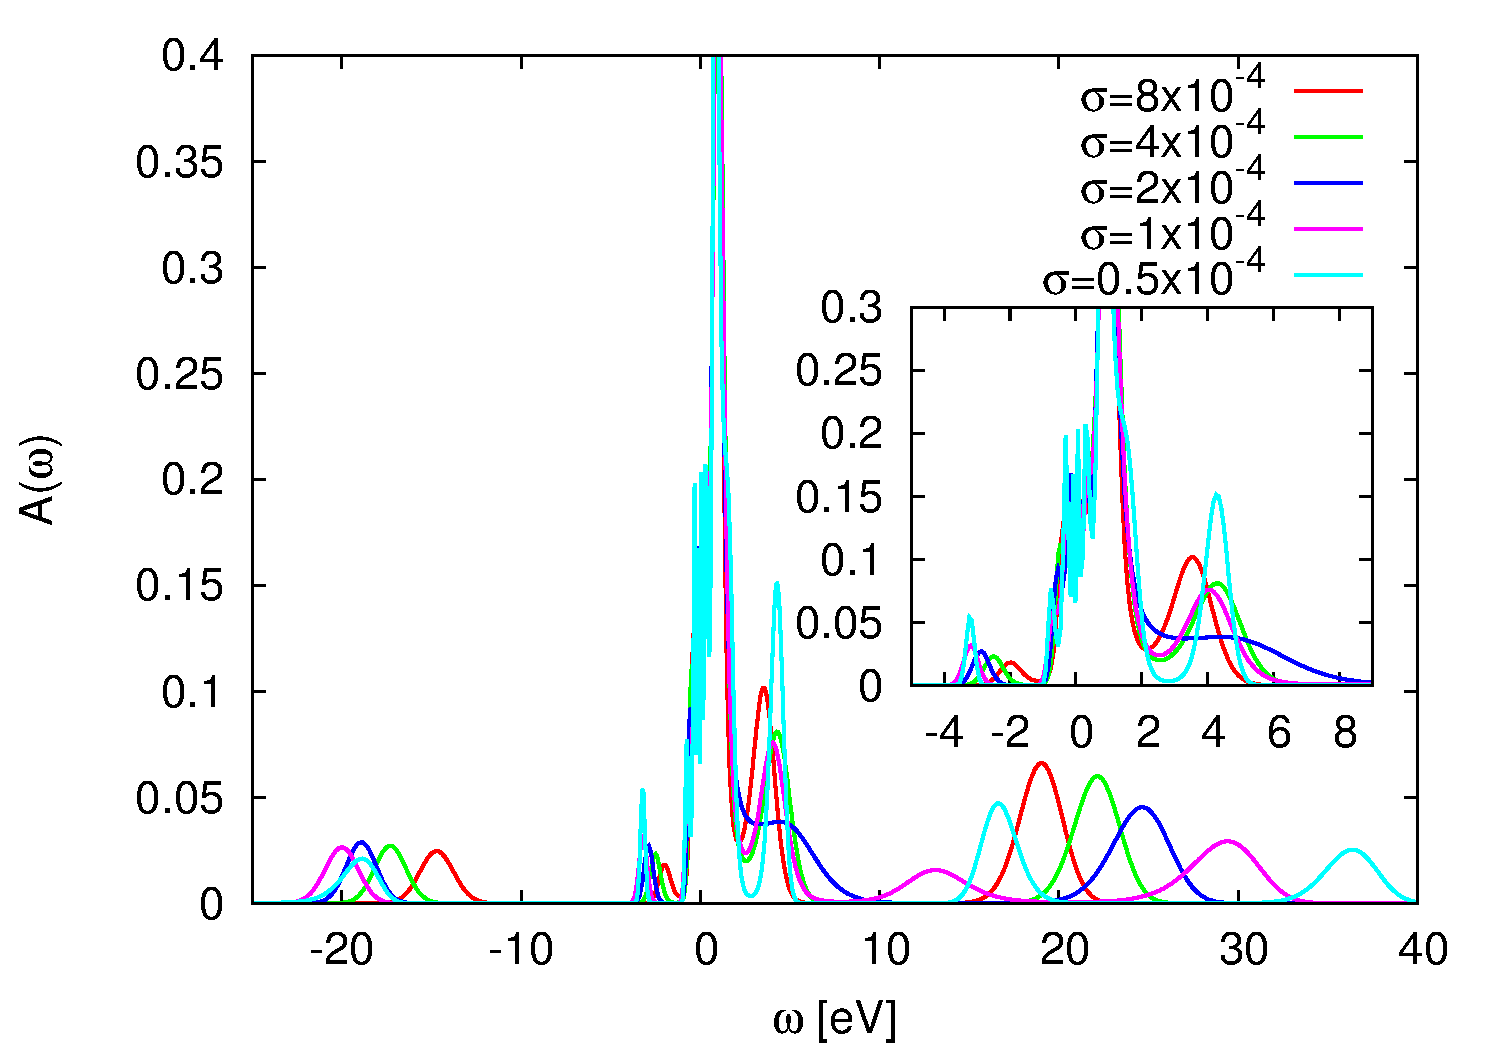
\includegraphics[width=0.9\textwidth]{figs/GW_maxent_diffSigma.pdf}
\caption{The spectral function from G$_0$W$_0$ (7x7x7 k-points) obtained from
Maxent, using a constant standard deviation $\sigma$. The Green's function
on the Matsubara axis $i\omega_n$ for 1000 frequenices at $\beta=40$\ 1/eV was continued
using a gaussian default model.}
\label{fig:gw_anacont_diff_sigma}
\end{figure}

The analytic continuation becomes increasingly hard for the case
of frequency dependent interactions $U(\omega)$,
since plasmonic features appear in the spectral function, resp.
Green's function at multiples of the plasma frequency,
for example in SrVO$_3$ $\omega_p\approx 15$~eV.
Therefore, the energy window has to be chosen considerably large, at least $\pm 3\omega_p$
to obtain a proper normalization of the spectral function.

At the same time the high-energy features cannot be accurately resolved because the
kernel that has to be inverted becomes very small at high energies
\begin{align}
G(i\omega_n) &= \frac{1}{\pi} \int_{-\infty}^{\infty} \mathrm{Im}[G(\omega)] 
                                \frac{1}{\omega-i\omega_n}\mathrm{d}\omega \\
G(\tau) &= \frac{1}{\pi} \int_{-\infty}^{\infty} \mathrm{Im}[G(\omega)]
                             \frac{\mathrm{e}^{-\tau\omega}}{\mathrm{e}^{-\beta\omega}+1}\mathrm{d}\omega.
\end{align}
Performing the analytic continuation from the Matsubara axis $i\omega_n$
should in principle be easier, since the Kernel $K(\omega,i\omega_n)= \frac{1}{\omega-i\omega_n}$
does decay significantly slower than the Kernel
$K(\omega,\tau)=\frac{\mathrm{e}^{-\tau\omega}}{\mathrm{e}^{-\beta\omega}+1}$
for the continuation to the imaginary time axis $\tau$.
Therefore, plasmonic features at large $\omega$ are less suppressed
by $K(\omega,i\omega_n)$ than by $K(\omega,\tau)$, so small changes on the real
frequency axis $\omega$ should be more visible in $G(i\omega_n)$ than in $G(\tau)$.

In practice I think it is still better to use Maxent with $G(\tau)$
directly measured at $\tau_i$, since the Legendre representation usually used
on both $\tau$ and $i\omega_n$ introduces very spurious correlated errors
in the measured quantities, where no good error estimate exist.
Only for $G(\tau)$ we have a well defined measure of the error bar 
which is measured in the solver and should be used for the Maxent input. 
Maybe one can use the direct measurement on $i\omega_n$ (more costly)
in the future?

\begin{figure}[t]
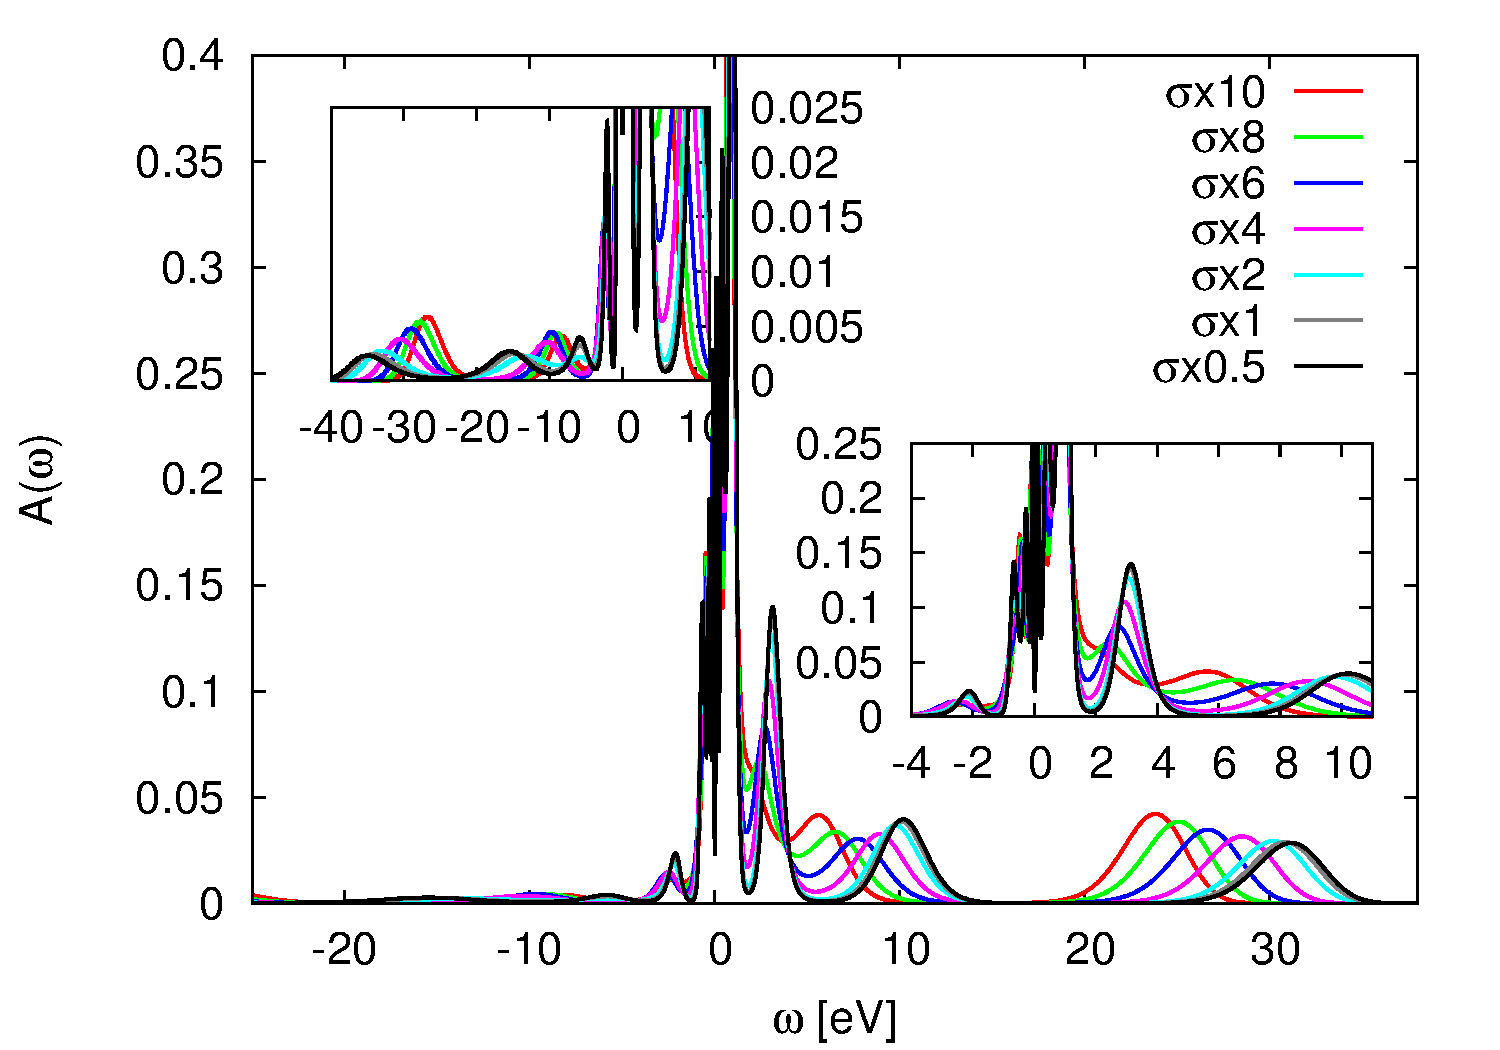
\includegraphics[width=0.9\textwidth]{figs/GWDMFT_maxent_diffSigma.pdf}
\caption{The spectral function from GW+DMFT (7x7x7 k-points) obtained from
Maxent, using the mesured standard deviation $\sigma(\tau)$
from the impurity solver. The Green's function
on the imaginary time axis $\tau$ for 2048 points at $\beta=40$\ 1/eV was continued
using a gaussian default model. The standard deviation was scaled by different
factors to show the dependence on $\sigma$. The factor 1 corresponds
to the initial value of $\sigma$ measured in the Monte Carlo Solver.}
\label{fig:gwdmft_anacont_diff_sigma}
\end{figure}

%%%%%%%%%%%%%%%%%%%%%%%%%%%%%%%%%%%%%%%%%%%%%%%%%%%%%%%%%%%%%%%%%%%%%%%%%%%%%%%%%%%%%
%%%%%%%%%%%%%%%%%%%%%%%%%%%%%%%%%%%%%%%%%%%%%%%%%%%%%%%%%%%%%%%%%%%%%%%%%%%%%%%%%%%%%
%%%%%%%%%%%%%%%%%%%%%%%%%%%%%%%%%%%%%%%%%%%%%%%%%%%%%%%%%%%%%%%%%%%%%%%%%%%%%%%%%%%%%
%%%%%%%%%%%%%%%%%%%%%%%%%%%%%%%%%%%%%%%%%%%%%%%%%%%%%%%%%%%%%%%%%%%%%%%%%%%%%%%%%%%%%
%%%%%%%%%%%%%%%%%%%%%%%%%%%%%%%%%%%%%%%%%%%%%%%%%%%%%%%%%%%%%%%%%%%%%%%%%%%%%%%%%%%%%

\section{Dependence on the k-mesh}
\begin{figure}[h]
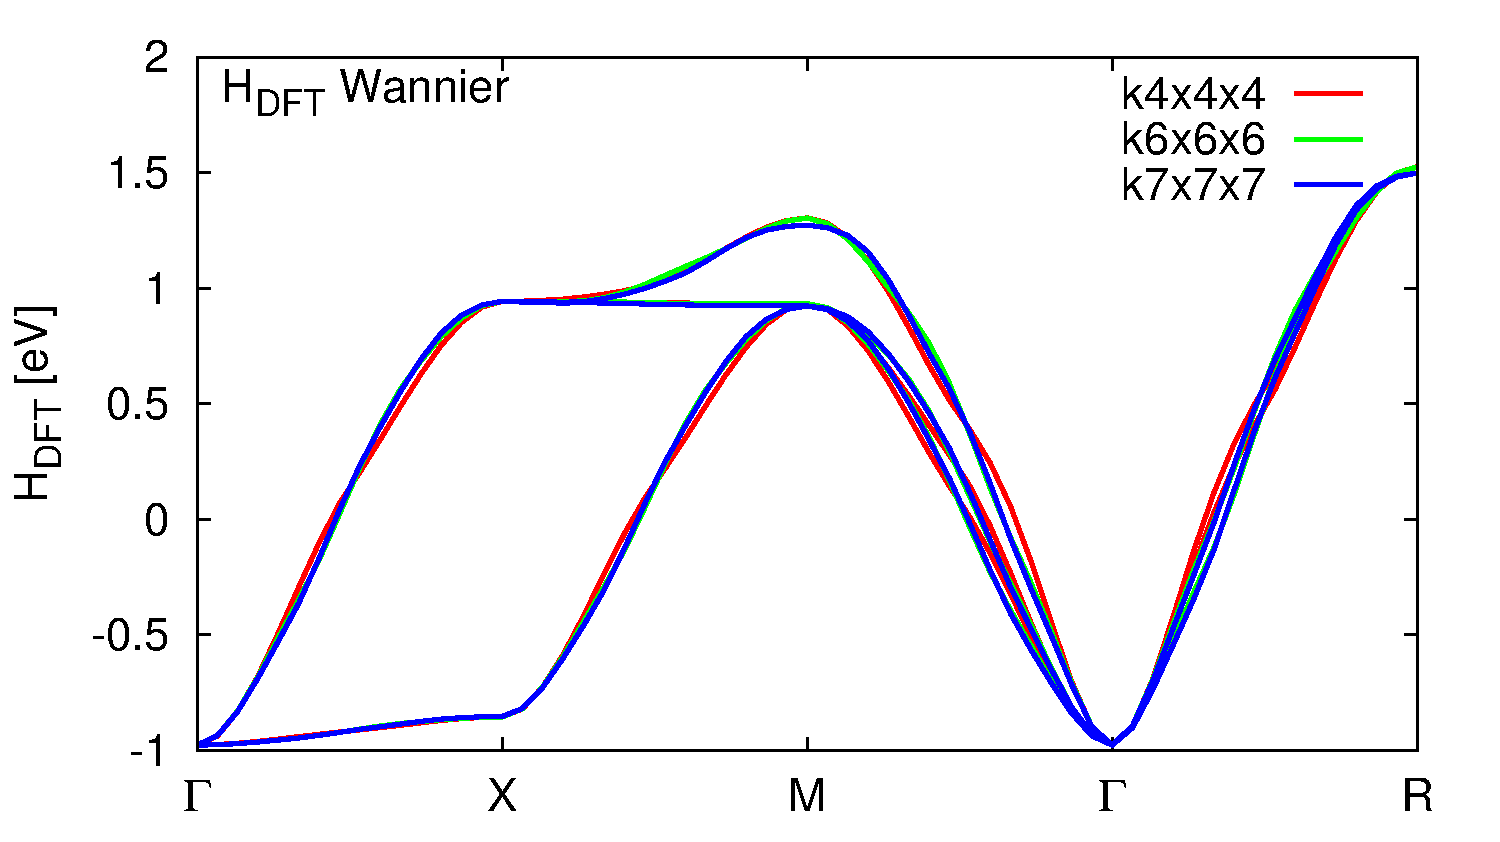
\includegraphics[width=0.5\textwidth]{figs/hdft_kpath.pdf}
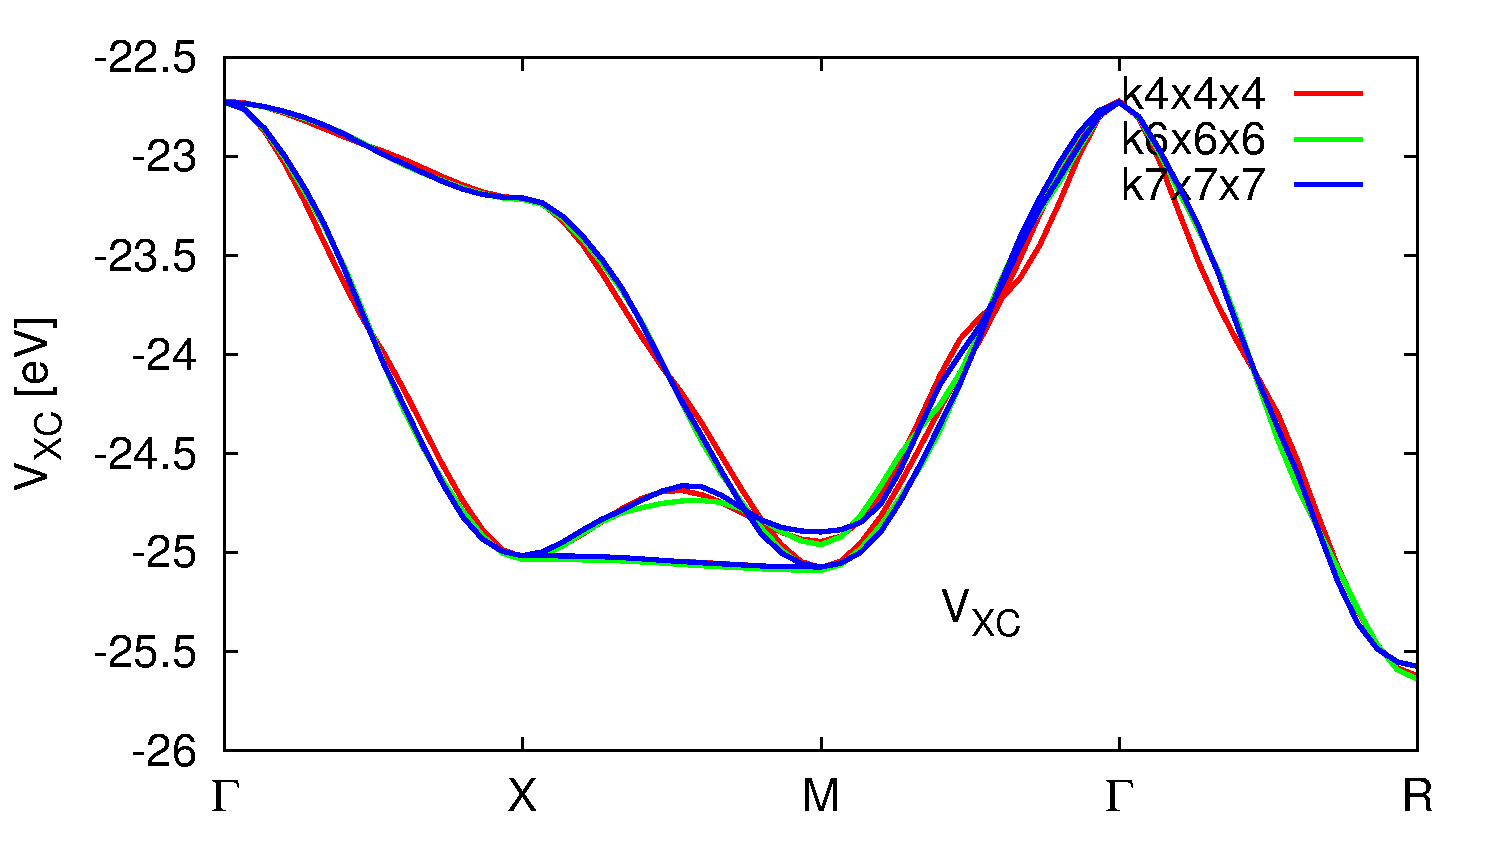
\includegraphics[width=0.5\textwidth]{figs/vxc_kpath.pdf}
\begin{center}
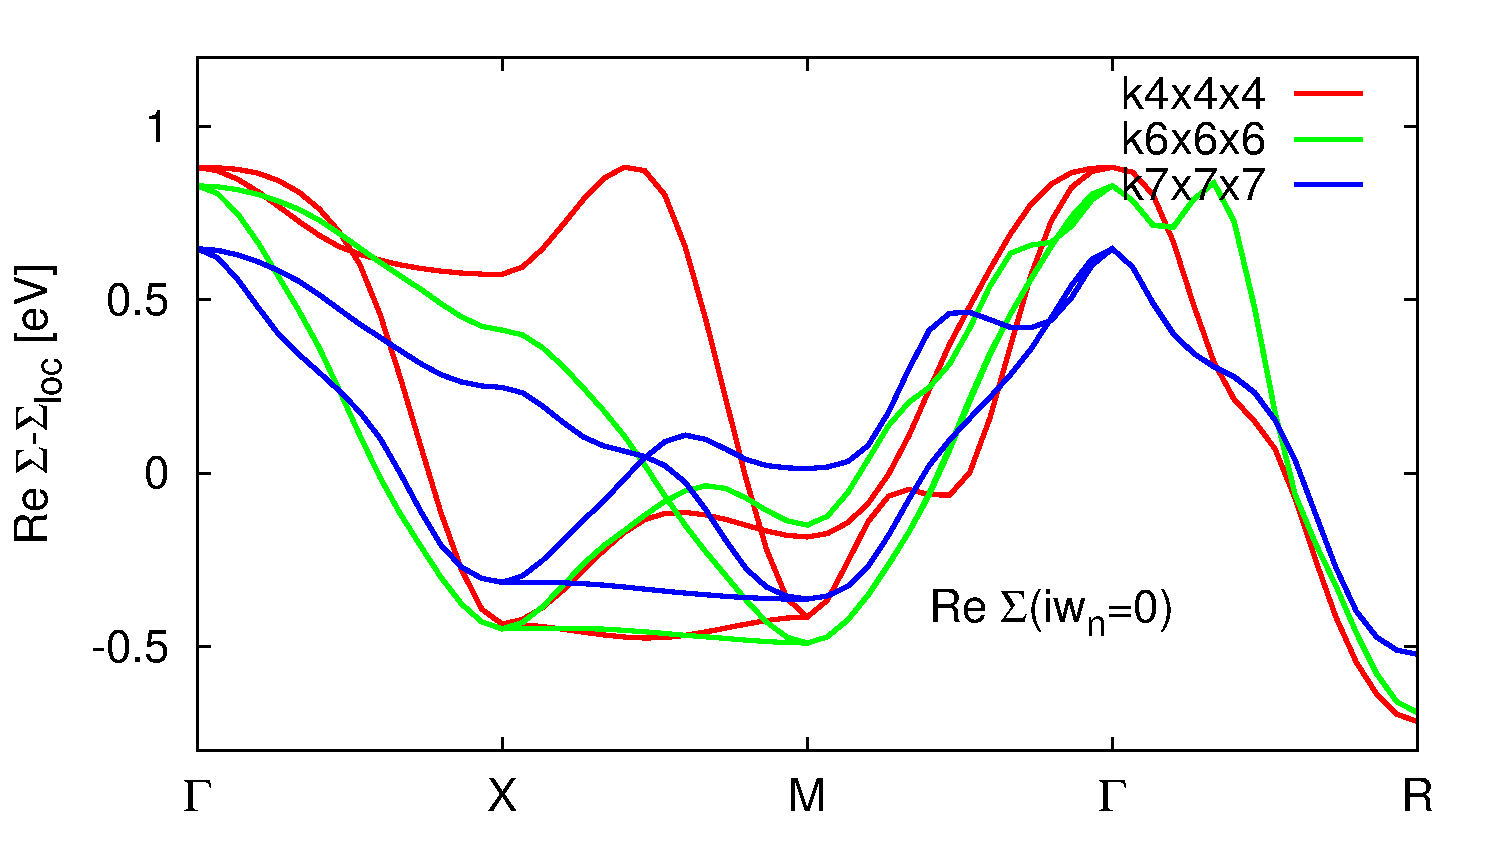
\includegraphics[width=0.7\textwidth]{figs/ReSigma_kpath.pdf}
\end{center}
\caption{Top: The Eigenvalues of the DFT tight-binding Hamiltonian $H_{DFT}$.\\
Middle: The exchange-correlation potential $V_{XC}$. \\
Bottom: The real part of the $G_0W_0$ Selfenergy at the lowest Matsubara frequency
at $\beta=40$\ 1/eV. }
\label{fig:gw_kpath_kmesh_comp}
\end{figure}

In Fig. \ref{fig:gw_kpath_kmesh_comp} we show 
the Eigenvalues of the DFT tight-binding Hamiltonian $H_{DFT}$,
the exchange-correlation potential $V_{XC}$ and the real part of the $G_0W_0$ 
Selfenergy at the lowest Matsubara frequency at $\beta=40$\ 1/eV
along a certain k-path. Calculations based on different k-meshes are compared.


All objects have been interpolated to a $30\times30\times30$ k-mesh,
starting from a $G_0W_0$ on different smaller k-grids. $H_{DFT}$ and $V_{XC}$ show basically
negligible variation for different number of k-points since their values are directly taken from
a DFT calculation converged on a much denser grid. The only variation is due
to the interpolation from the smaller to the larger grid, which becomes more accurate 
with higher number of k-points.\\
The Selfenergy has been shifted so that zero corresponds to the value of the
local Selfenergy for each calculation. Most of the difference is inherent
due to the small k-resolution of the $G_0W_0$ calculation and not due to the interpolation.
The difference between $6\times 6 \times 6$ and  $7\times 7 \times 7$ k-points
is still huge and a denser grid has to be considered for a proper
calculation (maybe $10\times 10 \times 10$ is enough? Check especially
for odd/even numbers!)


%%%%%%%%%%%%%%%%%%%%%%%%%%%%%%%%%%%%%%%%%%%%%%%%%%%%%%%%%%%%%%%%%%%%%%%%%%%%%%%%%%%%%
%%%%%%%%%%%%%%%%%%%%%%%%%%%%%%%%%%%%%%%%%%%%%%%%%%%%%%%%%%%%%%%%%%%%%%%%%%%%%%%%%%%%%
%%%%%%%%%%%%%%%%%%%%%%%%%%%%%%%%%%%%%%%%%%%%%%%%%%%%%%%%%%%%%%%%%%%%%%%%%%%%%%%%%%%%%
%%%%%%%%%%%%%%%%%%%%%%%%%%%%%%%%%%%%%%%%%%%%%%%%%%%%%%%%%%%%%%%%%%%%%%%%%%%%%%%%%%%%%
%%%%%%%%%%%%%%%%%%%%%%%%%%%%%%%%%%%%%%%%%%%%%%%%%%%%%%%%%%%%%%%%%%%%%%%%%%%%%%%%%%%%%

\section{Causality constraint}

\textbf{Definition:}
A Green's function $G$, Selfenergy $\Sigma$, or other functions $F$ derived from them
is called \textit{causal}, if 
\begin{align}
\mathrm{Im}F(\omega) \leq 0 \  \forall \omega \in \mathbb{R}.
\end{align}
\cng{Does it have to be strictly negative? }
For example, if a Green's function is causal then its related
spectral function $A(\omega) = -\mathrm{Im}G(\omega)/\pi \geq 0$.

\textbf{Theorem:}
A function $F(\omega)$ is causal if and only if its corresponding
transform $F(\tau)$ to the imaginary time interval $(0,\beta)$
has only negative definite even derivatives, i.e.
\begin{align}
F(\omega) \mbox{ causal }
%
\Leftrightarrow
%
\frac{\partial^{2n} }{\partial \tau^{2n}} F(\tau) \leq 0 \ \forall n\in\mathbb{N}.
\end{align}
\cng{Maybe its strictly negative?}

\textbf{Proof:}

$\Rightarrow$: Assume that $\mathrm{Im}F(\omega) \leq 0 \  \forall \omega \in \mathbb{R}$.
Using Cauchy's integral formula we have the relation
\begin{align}
F(i\omega_n) &= \frac{1}{\pi} \int_{-\infty}^{\infty} 
                \frac{\mathrm{Im}F(\omega)}{\omega - i\omega_n}\, \mathrm{d}\omega\\
%
F(\tau) &= \frac{1}{\pi} \int_{-\infty}^{\infty} 
          \mathrm{Im}F(\omega) \frac{\mathrm{e}^{-\tau\omega}}{\mathrm{e}^{-\beta\omega}+1}
          \, \mathrm{d}\omega                
\end{align}
The Kernel in the second expression 
$K(\tau,\omega) = \mathrm{e}^{-\tau\omega}/ \left( \mathrm{e}^{-\beta\omega}+1 \right)$
is strictly positive and  decays exponentially for
large $|\omega|$ for fixed $\tau\in (0,\beta)$
\begin{align}
\lim\limits_{\omega\rightarrow \infty} 
 \frac{\mathrm{e}^{-\tau\omega}}{\mathrm{e}^{-\beta\omega}+1}  
 &= \lim\limits_{\omega\rightarrow \infty} 
 \frac{\mathrm{e}^{-\tau\omega}}{0+1} \\
  &= 0 \\
 %
 %
 \lim\limits_{\omega\rightarrow -\infty} 
 \frac{\mathrm{e}^{-\tau\omega}}{\mathrm{e}^{-\beta\omega}+1}  
 &= \lim\limits_{\omega\rightarrow -\infty} 
 \frac{\mathrm{e}^{-\tau\omega}}{\mathrm{e}^{-\beta\omega}}   \\
 %
 &= \lim\limits_{\omega\rightarrow -\infty} 
\mathrm{e}^{(\beta-\tau)\omega} \\
&= 0.
\end{align}

In the limits $\tau=0$ or $\tau = \beta$ the Kernel $K(\tau,\omega)$ becomes the Fermi
distribution function for either negative or positive $\omega$
\begin{align}
 \lim\limits_{\tau\rightarrow 0}
 \frac{\mathrm{e}^{-\tau\omega}}{\mathrm{e}^{-\beta\omega}+1} 
 &=  \frac{1}{\mathrm{e}^{\beta(-\omega)}+1} \\
 %
 %
  \lim\limits_{\tau\rightarrow \beta}
 \frac{\mathrm{e}^{-\tau\omega}}{\mathrm{e}^{-\beta\omega}+1} 
 &= \frac{\mathrm{e}^{-\beta\omega}}{\mathrm{e}^{-\beta\omega}+1} \\
 &= \frac{1}{\mathrm{e}^{\beta\omega}+1}
\end{align}
For the derivatives $\partial_{\tau}^{2n} F(\tau) $ 
we get the expression
\begin{align}
\frac{\partial^{2n} }{\partial \tau^{2n}} F(\tau)
&=\frac{1}{\pi} \int_{-\infty}^{\infty} \mathrm{Im}F(\omega) 
 \frac{\partial^{2n} }{\partial \tau^{2n}}
          \frac{\mathrm{e}^{-\tau\omega}}{\mathrm{e}^{-\beta\omega}+1} \, \mathrm{d}\omega   \\
%             
&= \frac{1}{\pi} \int_{-\infty}^{\infty} \mathrm{Im}F(\omega) 
\omega^{2n}   K(\tau,\omega) \, \mathrm{d}\omega.
\end{align}
Since $\mathrm{Im}F(\omega) \leq 0 \  \forall \omega \in \mathbb{R}$,
the integral is also strictly non-positive.

\bigskip

$\Leftarrow$:

Do not investigate further since:
Using this for analytic continuation
does not work since any least-square fitting even without enforcing
the derivative constraints is too ill-behaved.


%%%%%%%%%%%%%%%%%%%%%%%%%%%%%%%%%%%%%%%%%%%%%%%%%%%%%%%%%%%%%%%%%%%%%%%%%%%%%%%%%%%%%
%%%%%%%%%%%%%%%%%%%%%%%%%%%%%%%%%%%%%%%%%%%%%%%%%%%%%%%%%%%%%%%%%%%%%%%%%%%%%%%%%%%%%
%%%%%%%%%%%%%%%%%%%%%%%%%%%%%%%%%%%%%%%%%%%%%%%%%%%%%%%%%%%%%%%%%%%%%%%%%%%%%%%%%%%%%
%%%%%%%%%%%%%%%%%%%%%%%%%%%%%%%%%%%%%%%%%%%%%%%%%%%%%%%%%%%%%%%%%%%%%%%%%%%%%%%%%%%%%
%%%%%%%%%%%%%%%%%%%%%%%%%%%%%%%%%%%%%%%%%%%%%%%%%%%%%%%%%%%%%%%%%%%%%%%%%%%%%%%%%%%%%



\section{Implementation details}

\subsection{Impurity solver input}

The CT-HYB impurity solver by Yusuke needs the following input files
\begin{description}
\item[dmft.input] Includes information about U,J, number of frequencies, etc. At the moment
possible: Only 3-fold degenerate orbitals. No freq. dependent U.

\item[hyb\_tau.dat] The hybridization function as a matrix for imaginary time. 
It needs to be diagonal! \\
Only real part, one column. Seperate matrix elements
via two line breaks and \verb|# hyb     2    1| etc. We need \verb|Nmesh+1|
points where the endpoints $\tau=0,\beta$ are included! By convention has negative sign.
\cng{The local orbital levels are assumed to be $\tilde{\mu}=0$ and any
shift is absorbed in the chemical potential! This has to 
be checked for consistency!!!}

\item[omega\_mesh.dat] Specifies the bosonic frequency grid for some 
correlation functions. Just reuse the standard template file. Not important for us.

\item[fort.10*] Includes information about the Monte-Carlo configuration used
for starting the sampling. Is initialized once with Yusuke's code and then overwritten by 
the solver. No change required here.
\end{description}

\clearpage

\subsection{Bandstructure calculation}
All data in the GW+DMFT calculation is given on the imaginary Matsubara frequency axis. To obtain 
the Bandstructure on real frequencies, we proceed as follows:
\begin{enumerate}
\item First, we create the Green's function for a given $k$-point on the Matsubara axis via
\begin{align}
 G(k,i\omega_n) 
 &= \left[ \unity(i\omega_n+\mu ) -H^{DFT}(k) + v^{XC}(k) \right. \nonumber \\
          & \hspace{1cm}- \Sigma^{GW}(k,i\omega_n) 
          + \Sigma^{GW,loc}(i\omega_n)
          \left. - \Sigma^{imp}(i\omega_n)
           \right]^{-1} 
%
\end{align}
Or, for example, to obtain only the GW Bandstructure we set the impurity contributions to zero
\begin{align}
 G(k,i\omega_n) 
 &= \left[ \unity(i\omega_n+\mu ) -H^{DFT}(k) + v^{XC}(k) \right. \nonumber \\
          &\left. \hspace{1cm}- \Sigma^{GW}(k,i\omega_n) 
           \right]^{-1} 
%
\end{align}
Then the Pade-approximation is applied to $G(k,i\omega_n) $ to obtain $G(k,\omega) $ on the real axis.
This is done for all k-points.
The spectral function is then given by
\begin{align}
A(k,\omega) = -\frac{1}{\pi} \mathrm{Im}G(k,\omega)
\end{align}

\end{enumerate}


\end{document}
